%%%%%%%%%%%%%%%%%%%%%%%%%%%%%%%%%%%%%%%%%%%%%%%%%%%%%%%%%%%%%%%%%%%%%%%%%%%%%%%%%%%%%%
%																		 			%%
%																		 			%%
%																		 			%%
%																		 			%%
%						Document: Written by Marly Tatiana Celis Galvez 			%%
%						Assignment Part I Time Series Applied Macroeconometrics		%%
%																		 			%%
%																		 			%%
%																		 			%%
%%%%%%%%%%%%%%%%%%%%%%%%%%%%%%%%%%%%%%%%%%%%%%%%%%%%%%%%%%%%%%%%%%%%%%%%%%%%%%%%%%%%%%
\documentclass[11pt]{article}
\usepackage[T1]{fontenc}
\usepackage[margin=70pt]{geometry}

%References
\usepackage[style=authoryear,sorting=nyt,backend=biber]{biblatex}
		%\addbibresource{D:/Thesis/to_overleaf.bib}
%
%\usepackage{shellesc}
\usepackage{minted}
%[cache=false]
%		
\usepackage{standalone}
\usepackage[hidelinks]{hyperref}
\usepackage{csquotes}    
%When using babel or polyglossia with biblatex, loading csquotes is recommended 
%to ensure that quoted texts are typeset according to the rules of your main language.

%Math packages
\usepackage{amsfonts,latexsym,amsthm,amssymb,amsmath,amscd,euscript}
\usepackage{mathtools}
%Images packages
\usepackage{float}
\restylefloat{table}
\usepackage{tikz}
\usetikzlibrary{positioning}

\usepackage{array}
\usepackage{multirow}
\usepackage{xcolor}
\usepackage{tabularx,ragged2e,booktabs,caption}
\newcolumntype{P}[1]{>{\centering\arraybackslash}p{#1}}
%\usepackage{caption}
\usepackage{subcaption}
\usepackage{float}
%\pagestyle{fancy}

	\usepackage{fancyhdr}
	\pagestyle{fancy}
	\fancyhf{}
	\rhead{Marly Tatiana Celis}
	\lhead{Groningen University - Utretch University}
	\lfoot{\href{mailto:m.t.celis.galvez.1@student.rug.nl}{{\tt m.t.celis.galvez.1@student.rug.nl}}}

%$ latex -shell-escape input
%																		 			%%
%																		 			%%
%																		 			%%
%																		 			%%
%%%%%%%%%%%%%%%%%%%%%%%%%%%%%%%%%%%%%%%%%%%%%%%%%%%%%%%%%%%%%%%%%%%%%%%%%%%%%%%%%%%%%%
%																		 			%%
%																		 			%%
%																		 			%%
\begin{document}
%																		 			%%
%																		 			%%
%																		 			%%
%%%%%%%%%%%%%%%%%%%%%%%%%%%%%%%%%%%%%%%%%%%%%%%%%%%%%%%%%%%%%%%%%%%%%%%%%%%%%%%%%%%%%%
\begin{center} 
	\Large Applied Macroeconometrics 2021 \\
	Assignment Part I Time series econometrics
\end{center} 
%%%%%%%%%%%%%%%%%%%%%%%%%%%%%%%%%%%%%%%%%%%%%%%%%%%%%%%%%%%%%%%%%%%%%%%%%%%%%%%%%%%%%%

This document contains my solutions for the assignment 1 for the course Applied Macro Econometrics 2021, an elective taken at Groningen University. \\
\indent Marly Tatiana Celis Galvez \\
\indent Research Master - Multidisciplinary Economics \\
\indent Utrecht University

\tableofcontents






%%%%%%%%%%%%%%%%%%%%%%%%%%%%%%%%%%%%%%%%%%%%%%%%%%%%%%%%%%%%%%%%%%%%%%%%%%%%%%%%%%%%%%
\newpage
\section{Exercise 1}

Multivariate time series modelling\\

Aruba is a island and a constituent country of the Netherlands in the southern Caribean sea. Before COVID-19, about three-quarters of the Aruban gross national product was earned through tourism and related activities. Most tourists cam from North America, with a market-share of 73.3\%, followed by Latin America with 15.2\% and Europe with 8.3\%. The spreadsheet tourism series.xlsx has monthly series of stay-over visitors, visitor's nights, cruise visitors and ship calls.

\subsection{Descriptive part}
\subsubsection{Informative graphs}
Design informative graphs of and describe patterns in the series of cruise visitors and stay-over visitors to Aruba
For the first question I will plot the series. Perhaps, I'll try to observe the components of the series, for example, the trend, the  cycle, the seasonality, and the irregular part. At the least, I will discuss it. \\
In addition,  I can graph some correlograms \\

Before I can tell something about modelling the relationship between the two variables, I graphed the series to look for visible problems with the series. Such problems can include seasonal patterns, abrupt changes, discontinuities, and outliers. 
%Changes in the seasonal pattern that occur sufficiently far back in the past can be avoided sumpy by advancing the starting date of the used for adjustment or for modeling.
\begin{figure}[h!]
    \centering
    \begin{subfigure}[t]{0.45\textwidth}
         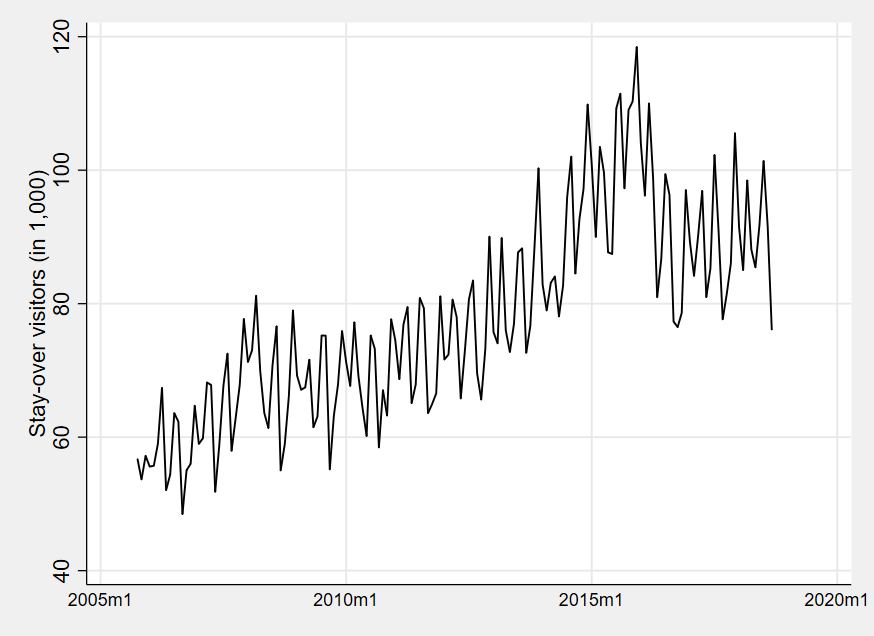
\includegraphics[width=\textwidth]{plots_1/lStayovervisitorsin1000.png}
    \end{subfigure}
    \begin{subfigure}[t]{0.45\textwidth}
          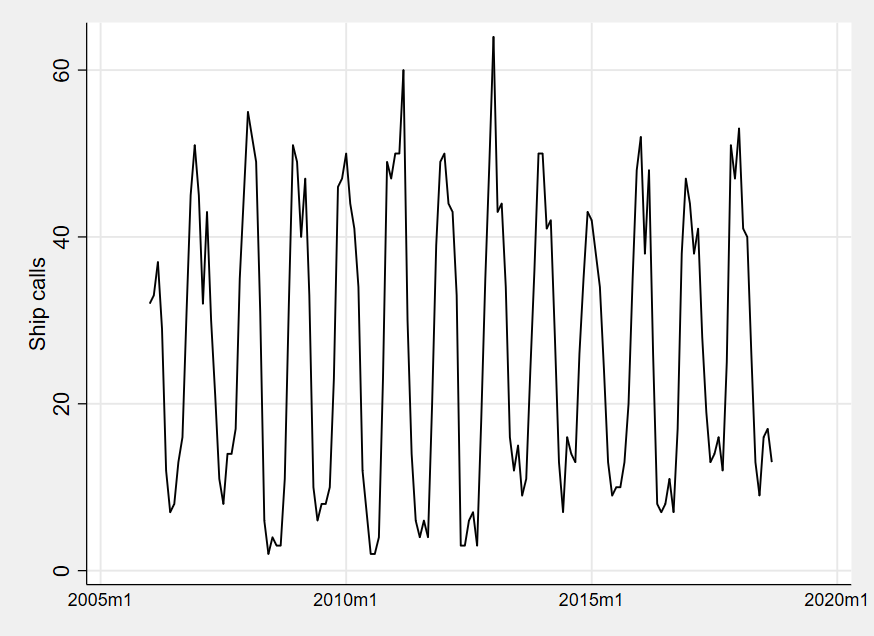
\includegraphics[width=\textwidth]{plots_1/lShipcalls.png}
    \end{subfigure}
    \begin{subfigure}[b]{0.45\textwidth}
          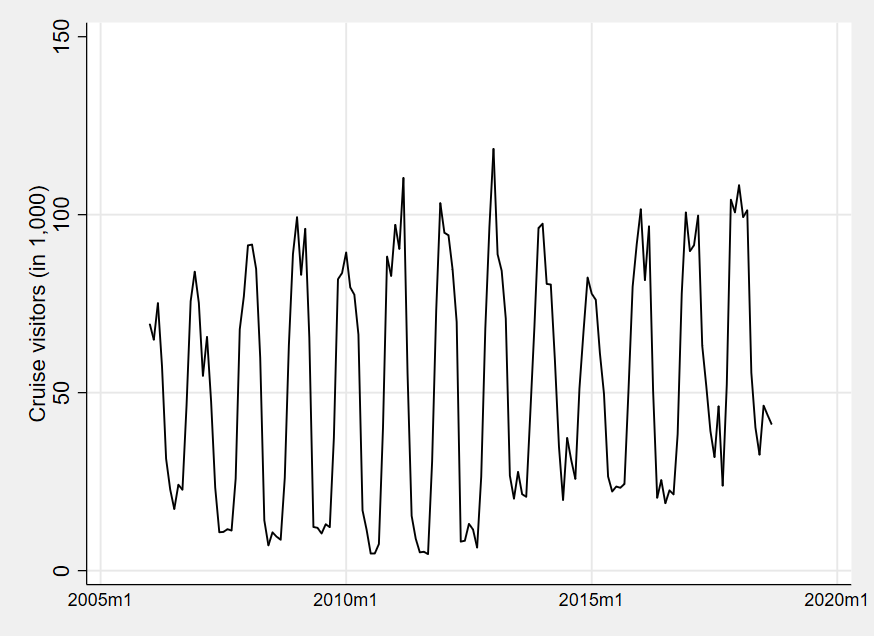
\includegraphics[width=\textwidth]{plots_1/lCruisevisitorsin1000.png}
    \end{subfigure}
        \begin{subfigure}[b]{0.45\textwidth}
        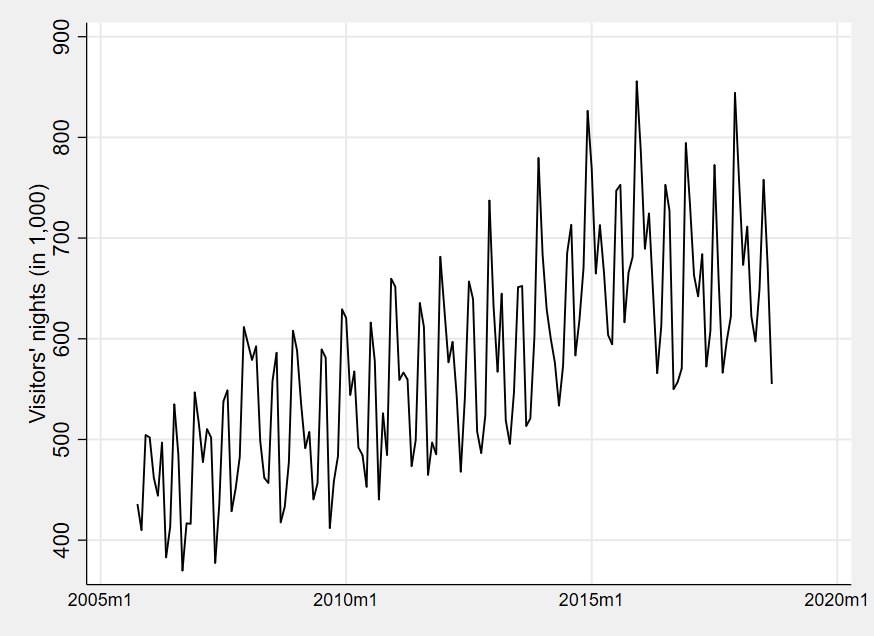
\includegraphics[width=\textwidth]{plots_1/lVisitorsnightsin1000.png}
    \end{subfigure}
    % \begin{subfigure}[b]{0.3\textwidth}
    %       \includegraphics[width=\textwidth]{Project_2/imgs/2/graph0.4.png}
    % \end{subfigure}
    % \begin{subfigure}[b]{0.3\textwidth}
    %       \includegraphics[width=\textwidth]{Project_2/imgs/2/graph1.png}
    % \end{subfigure}
    \caption{Series Tourism Aruba 2005-2018}
    \label{fig:originalseries}
\end{figure}


The corrgram command lists a table of autocorrelations, partial autocorrelations,
and Q statistics. It will also list a character-based plot of the autocorrelations and
partial autocorrelations


\begin{figure}[h!]
    \centering
    \begin{subfigure}[t]{0.45\textwidth}
         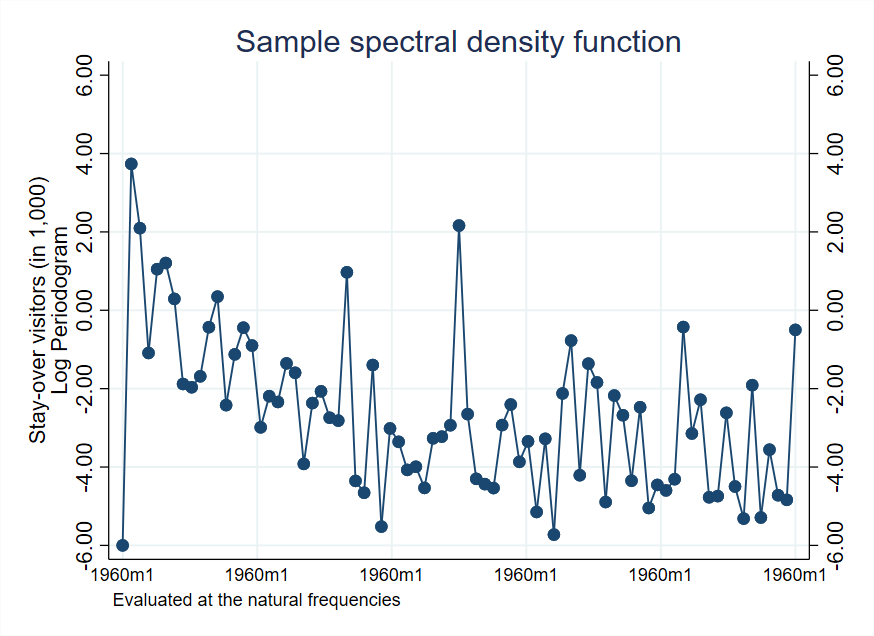
\includegraphics[width=\textwidth]{plots_1/pergram_1.png}
    \end{subfigure}
    \begin{subfigure}[t]{0.45\textwidth}
          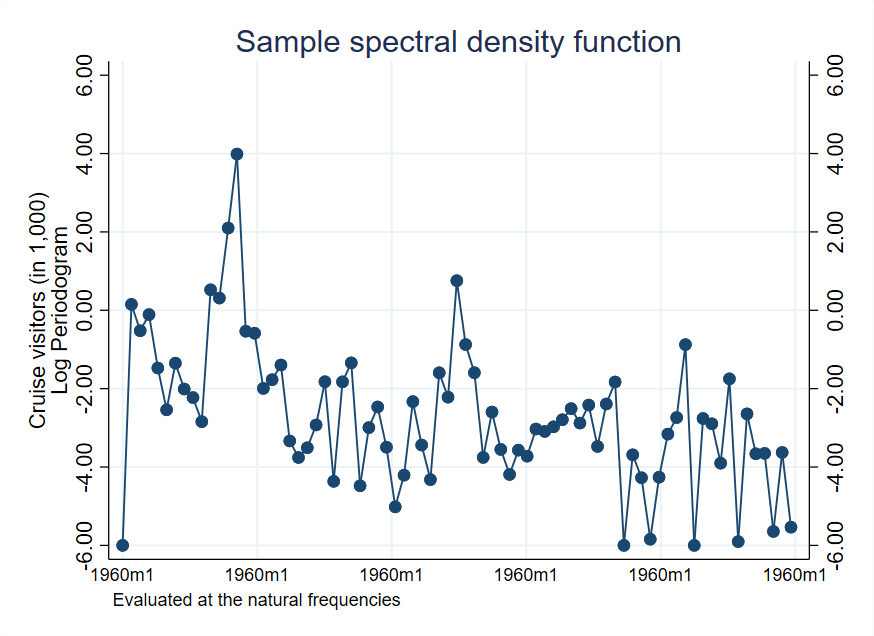
\includegraphics[width=\textwidth]{plots_1/pergram_2.png}
    \end{subfigure}
    \caption{Series Tourism Aruba 2005-2018}
    \label{fig:pergrams}
\end{figure}


Autocorrelation function

\begin{figure}[H]
    \centering
    \begin{subfigure}[t]{0.45\textwidth}
         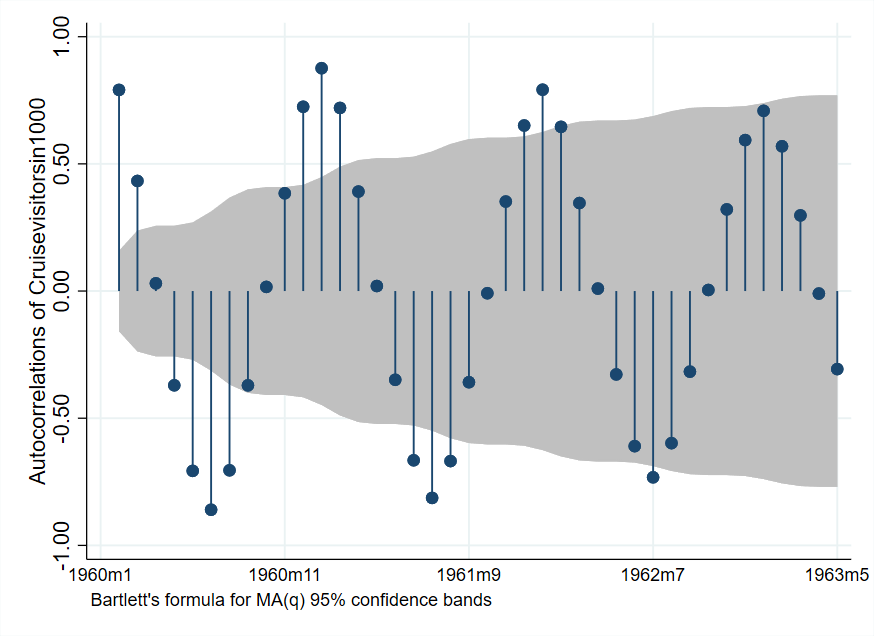
\includegraphics[width=\textwidth]{plots_1/cruise_ac_1.png}
    \end{subfigure}
    \begin{subfigure}[t]{0.45\textwidth}
          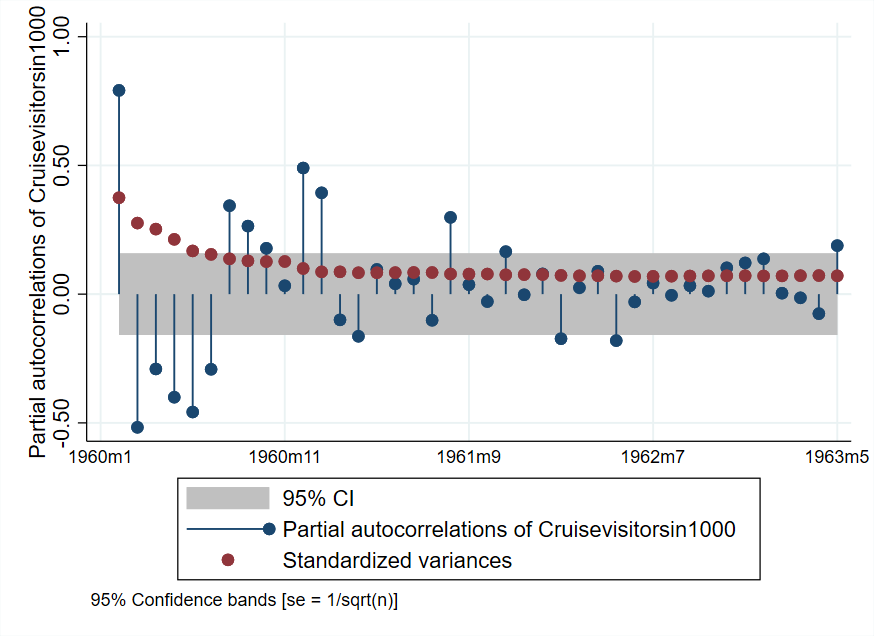
\includegraphics[width=\textwidth]{plots_1/cruise_pac_1.png}
    \end{subfigure}
    \begin{subfigure}[t]{0.45\textwidth}
         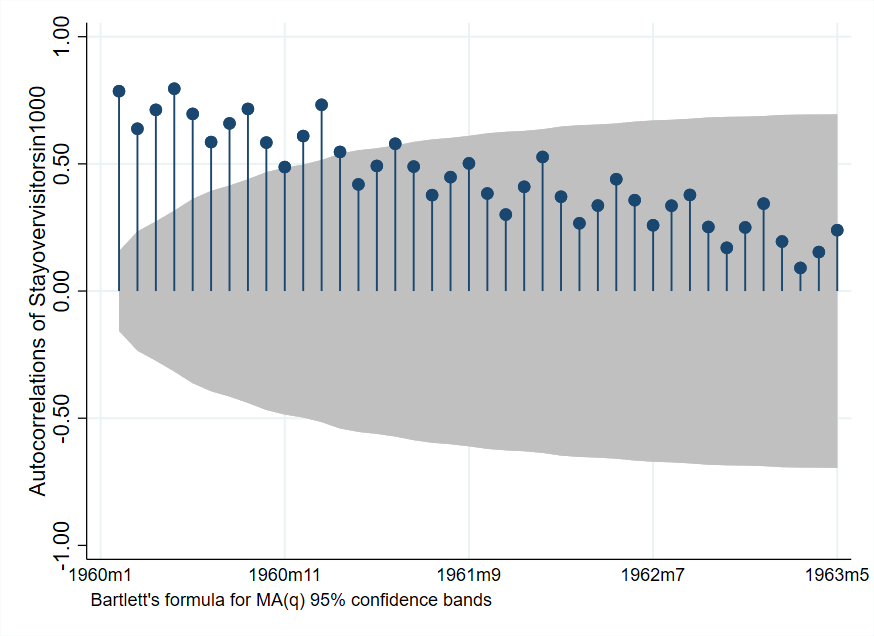
\includegraphics[width=\textwidth]{plots_1/stay_ac_1.png}
    \end{subfigure}
    \begin{subfigure}[t]{0.45\textwidth}
          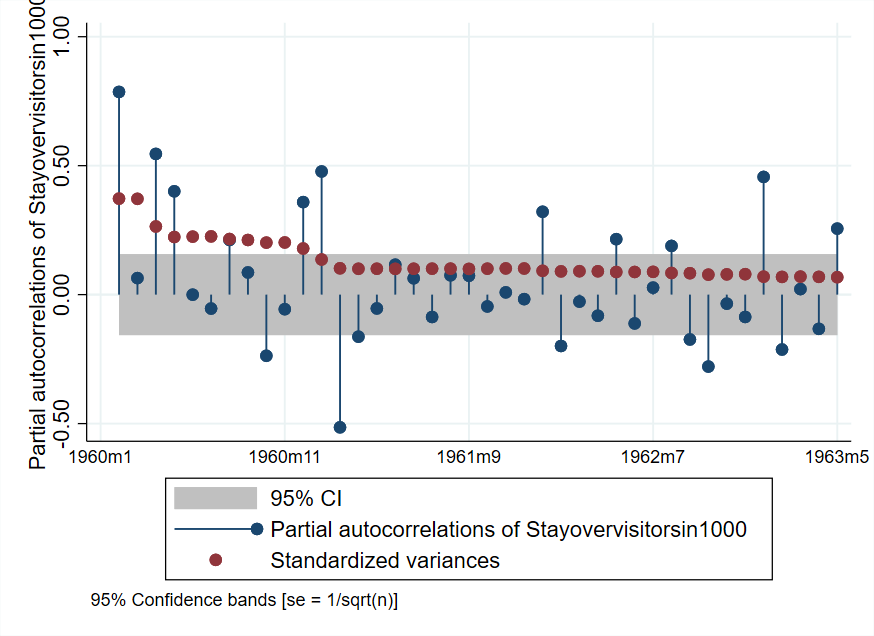
\includegraphics[width=\textwidth]{plots_1/stay_pac_1.png}
    \end{subfigure}
    \caption{AC and PACF 2005-2018}
    \label{fig:autorro}
\end{figure}

\begin{figure}[H]
    \centering
    \begin{subfigure}[t]{0.45\textwidth}
         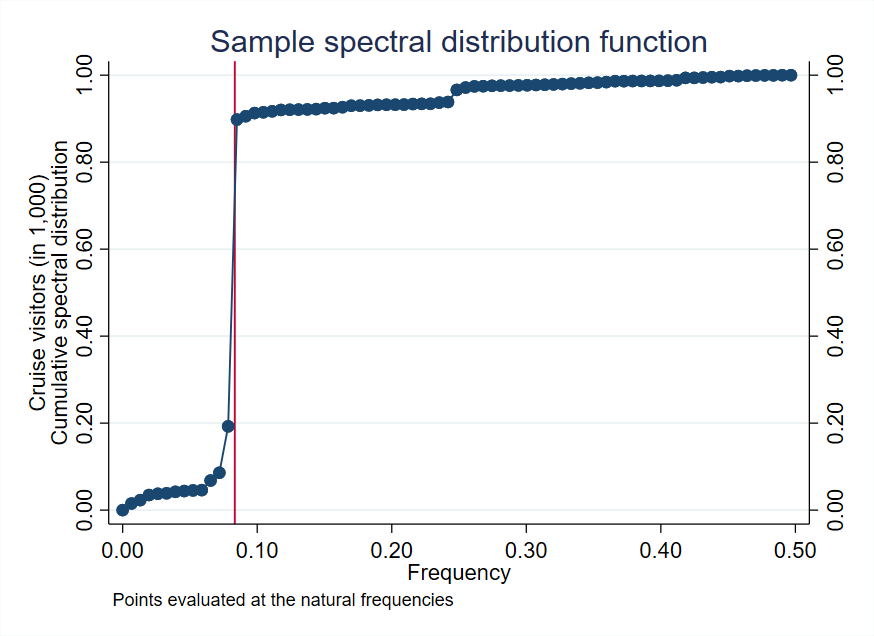
\includegraphics[width=\textwidth]{plots_1/cruise_spect_1.png}
    \end{subfigure}
    \begin{subfigure}[t]{0.45\textwidth}
          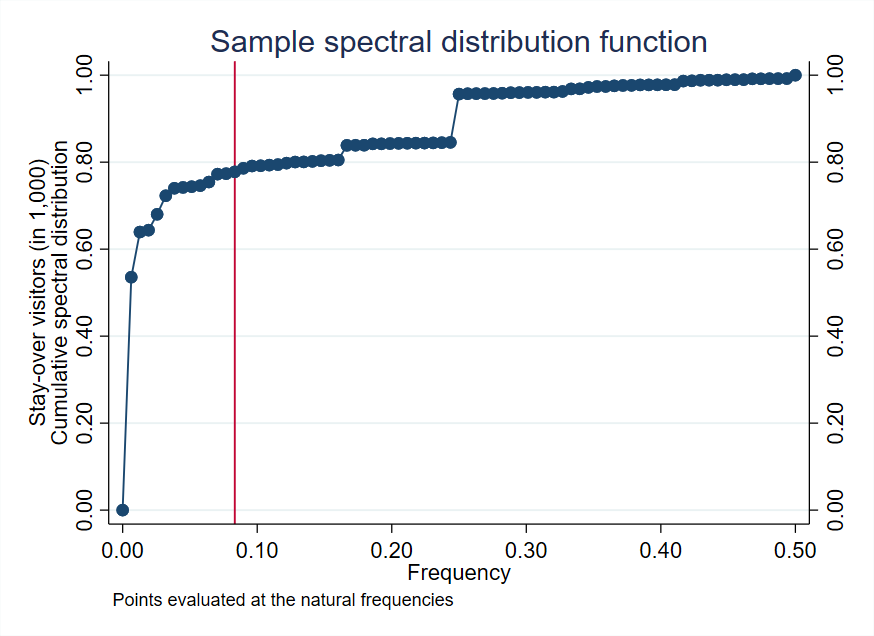
\includegraphics[width=\textwidth]{plots_1/stay_spect_1.png}
    \end{subfigure}
    \caption{Series Tourism Aruba 2005-2018}
    \label{fig:sepctral}
\end{figure}

\subsubsection{Modelling}
How would you proceed modelling the relationship between the two variables?. \\

For this second question, I would suggest to estimate a VAR model. A VAR model fits multivariate time-series regression of each of two series of our interest.\\
I would also take several steps:
\begin{itemize}
    \item Discount the seasonal component first. The main reason I would do so is because the series are related to tourism, which is in itself a phenomena that is related with seasonal changes. Particularly, monthly changes. For instance, it is well know that in tourism there are the so-called hot seasons, which are a time of the year when the number of people that prefer to spend their vacation on warmer places increases. Consequently, I expect that the behaviour of these series is affected by those kind of seasonal components.
    \item I should establish whether the series are non stationary. A stationary process is such that the mean, variances and covariances of the disturbances term $\epsilon_t$ do not change over time. Once I define the stationary process I will be sure that I am not finding spurious relations between the two series. 
%a process is said to be stationary if its probability distribution remains unchanged as time progresses
    \item I would also check whether the stationary process are cointegrated. As we know, when two $I(1)$ variables are cointegrated, or it exists a particular linear combination of these nonstationanry variables which is stationary. Indeed, cointegrated models stand that "In such cases a long-run relationship between these variables exists". The existence of a long-run relationship also has its implications for the short-run behaviour of the $I(1)$ variables, because there has to be some mechanism that drive the variables to their long-run equilibrium relationship.
\end{itemize}

I graph the two series without any adjustment, as shown in \ref{fig:behavriora} and \ref{fig:behavriorb}. However the seasonal component is strong and do not allow to perceive a clear relationship.
\begin{figure}[h!]
    \centering
    \begin{subfigure}[t]{0.45\textwidth}
         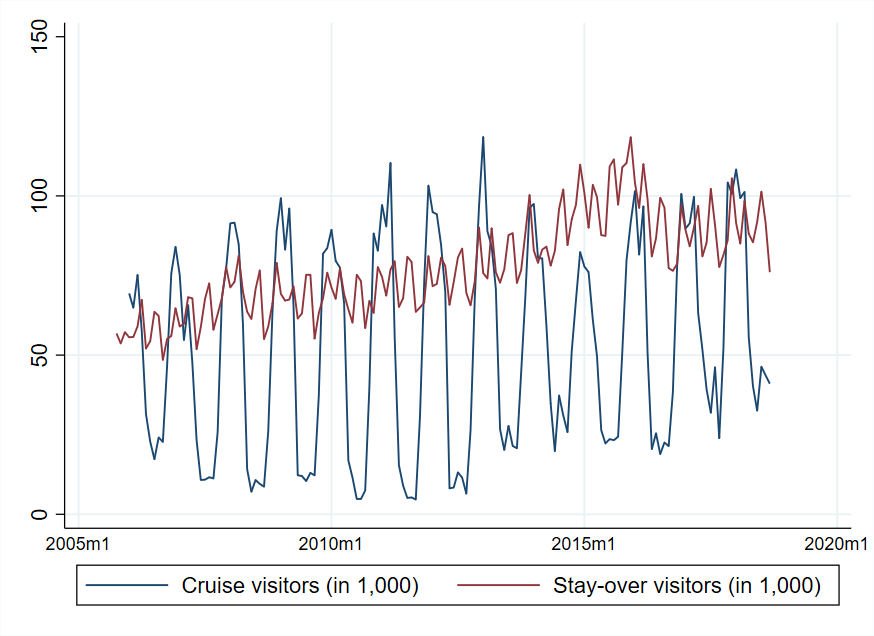
\includegraphics[width=\textwidth]{plots_1/orginal_nologs.png}
         \caption{Series Tourism Aruba 2005-2018 in Levels}
         \label{fig:behavriora}
    \end{subfigure}
    \begin{subfigure}[t]{0.45\textwidth}
          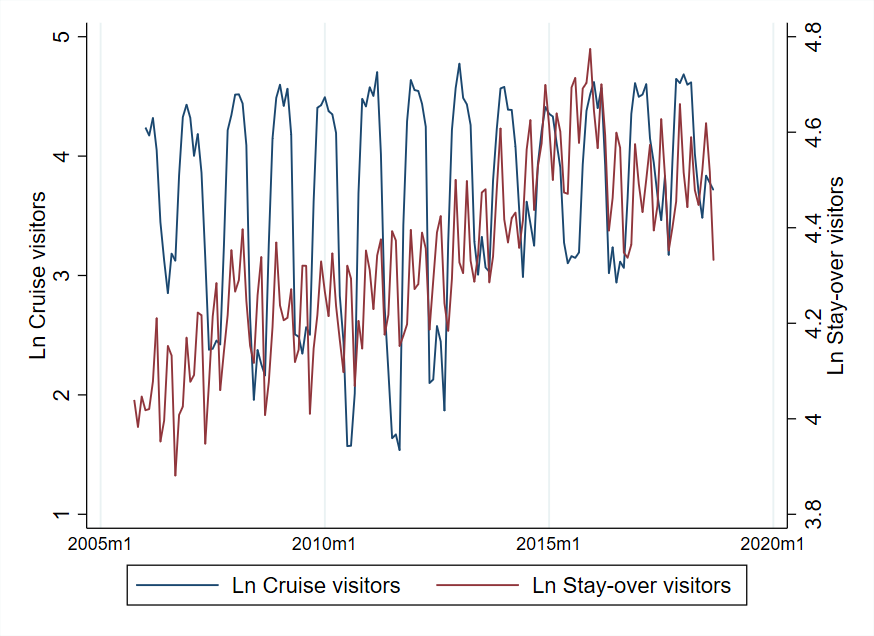
\includegraphics[width=\textwidth]{plots_1/series_originales.png}
          \caption{Series Tourism Aruba 2005-2018 in Logs}
    \label{fig:behavriorb}
    \end{subfigure}
\end{figure}
The scatter plot of the two series reveals a potential statistical relationship.
\begin{figure}[h!]
    \centering
     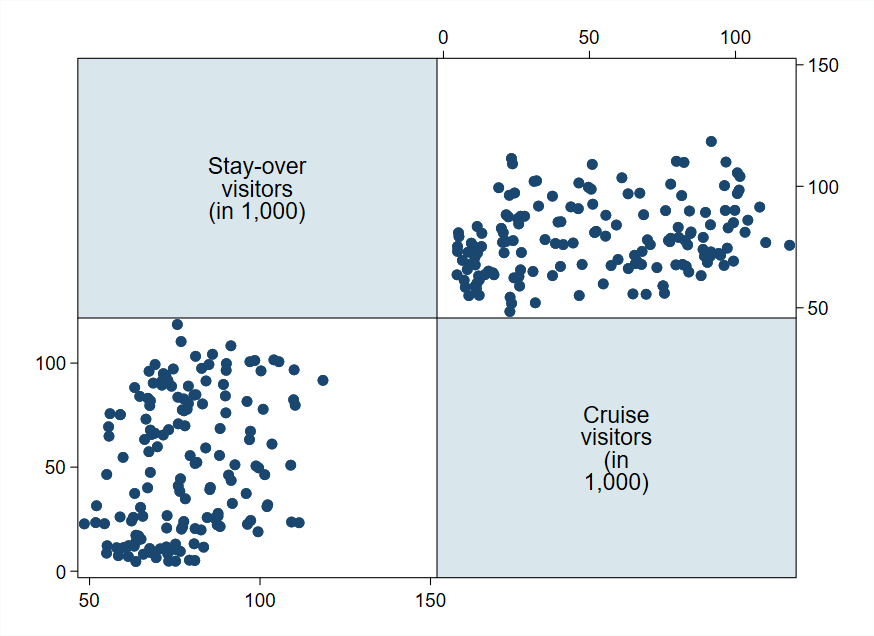
\includegraphics[width=0.6\textwidth]{plots_1/correlation_1.png}
     \caption{Scatter Plot - Series Tourism Aruba 2005-2018}
    \label{fig:scatter}
\end{figure}

\newpage
\subsection{Seasonality study}
For this part of the exercise I calculate natural logarithms and apply the seasonal adjustment filters X-13 ARIMA SEATS and CAMPLET to the two visitors series.
%To solve this exercise then I calculate the logarithm in excel for camplet
%And I use the file series.xlsx which contains only the two series of interest: cruise vistors and stayover visitors
% \begin{itemize}
% \item Compare outcomes for the seasonally adjusted series data
% \item Do the seasonal adjustment filters produce similar seasonal patterns?
% \item What happens if the last year of quarterly observations is discarded in the seasonal adjustment?
% \item Do the seasonally adjusted data lead to changes in your modelling approach described above?
% \end{itemize}

\subsubsection{Seasonal Adjustment with Camplet}
The objective is to get as high an accuracy percentage as possible. As a rule of thumb an accuracy over 60% gives reliable short extrapolations

\begin{table}[H]
\centering
\captionof{table}{CAMPLET Adjustment Results} \label{tab:title} 
\begin{tabular}{ l| c|c|c|c|c|c }
\toprule[1.25pt]
Series & Accuracy & Common adjustment & Multiplier & Pattern & LE & T \\
\midrule
Cruise visitors & 58 & 1.5 & 50 & 1 & 8 & 1 \\
Stay over visitors & 81 & 	1.5 & 50 & 1 & 8 & 1 \\
LN Cruise visitors & 76 & 	1.5 & 50 & 1 & 8 & 1 \\
LN Stay over visitors & 95 & 	1.5 & 50 & 1 & 8 & 1\\
\bottomrule[1.25pt]
\end{tabular}
\par
\end{table}

%Charts
% cam_crui_1.png cam_crui_2.png
% cam_stay_1.png cam_stay_2.png
\begin{figure}[H]
    \centering
    \begin{subfigure}[t]{0.45\textwidth}
         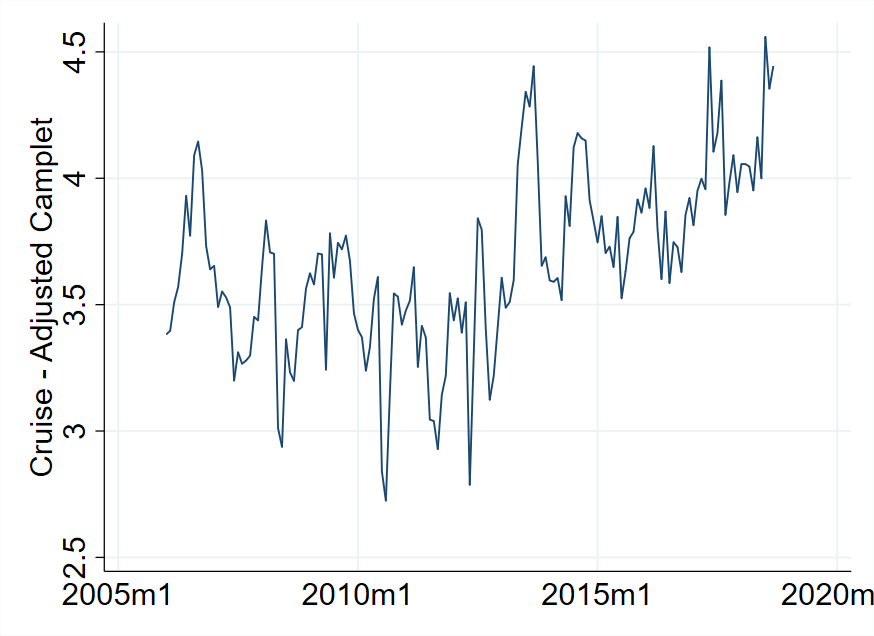
\includegraphics[width=\textwidth]{plots_1/cam_crui_1.png}
    \end{subfigure}
    \begin{subfigure}[t]{0.45\textwidth}
          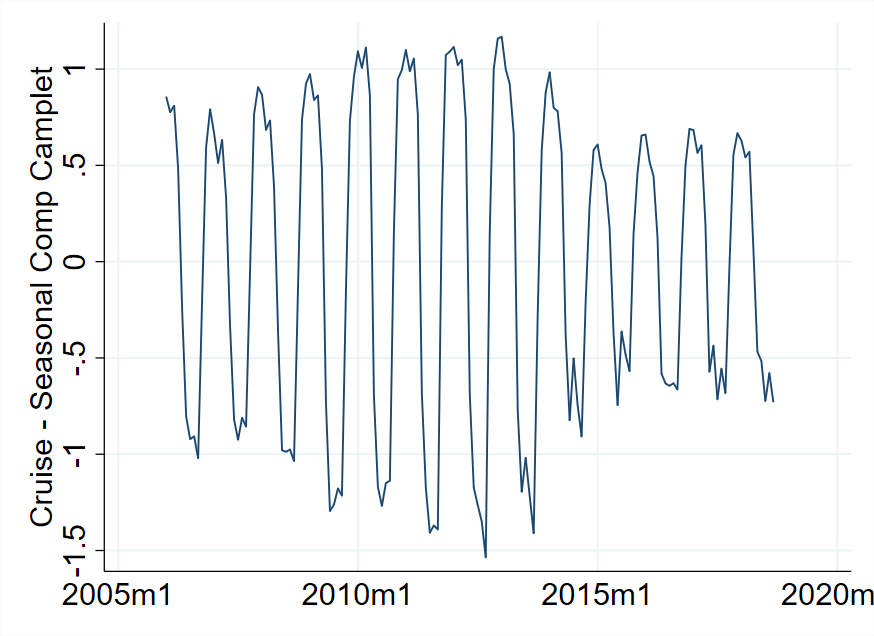
\includegraphics[width=\textwidth]{plots_1/cam_crui_2.png}
    \end{subfigure}
    \begin{subfigure}[t]{0.45\textwidth}
         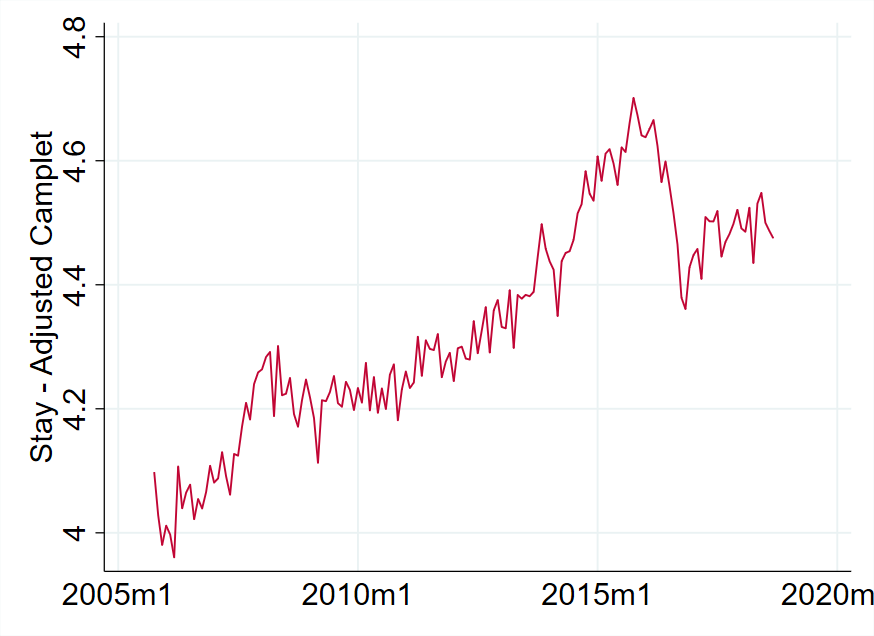
\includegraphics[width=\textwidth]{plots_1/cam_stay_1.png}
    \end{subfigure}
    \begin{subfigure}[t]{0.45\textwidth}
          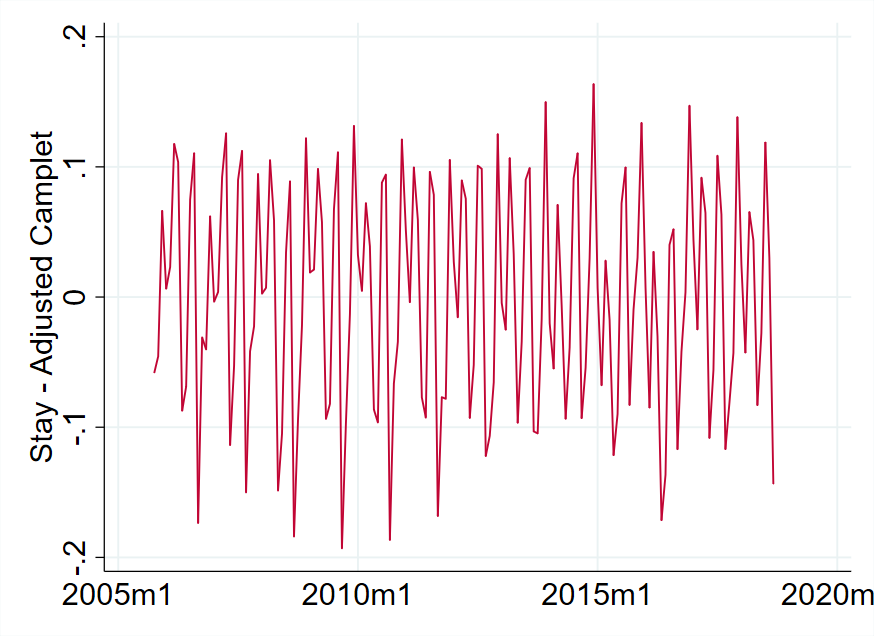
\includegraphics[width=\textwidth]{plots_1/cam_stay_2.png}
    \end{subfigure}
    \caption{Seasonal components for Cruise series using X-13 Arima Seats}
    \label{fig:campletadj1}
\end{figure}

Interpretation:
\begin{itemize}
\item Accuracy. The efficacy of extrapolations is high. Both of the series have an accuracy over 60\%; hence, it is possible to say that the adjustment has reliable short extrapolations.
\item Common adjustment. The applied length of the series is 1.5 years.
\item Multiplier. The applied length is 50 times the percentage deviation of the extrapolation from the measured value.
\item Pattern. The pattern is one year.
\item Limit to error. The tolerance of deviation beyond the series' path is 8\%.
\item Time. How often an outlier must return in corresponding periods to be dubbed a shift of pattern is 1.
\end{itemize}


\subsubsection{Seasonal Adjustment with X13 Arima Seats}
I downloaded the exectuable \textbf{X13Data.exe} from \href{https://www.census.gov/srd/www/x13as/}{www.census.gov}
%
% Contains a subdirectory named x13as with the following contents:
% the program x13as.exe (the X-13ARIMA-SEATS executable),
% a sample input file named testairline.spc,
% the Reference Manual and PC Quick Reference in a subdirectory named docs,
% and two Icon programs to assist users of X-13ARIMA-SEATS in a subdirectory named tools: genhol.exe (which generates user-defined regressors for moving holidays) and cnvx13as.exe (which converts spec files used with X-12-ARIMA to files that can be used with X-13ARIMA-SEATS), along with their documentation.
\begin{figure}[h!]
    \centering
    \begin{subfigure}[t]{0.45\textwidth}
         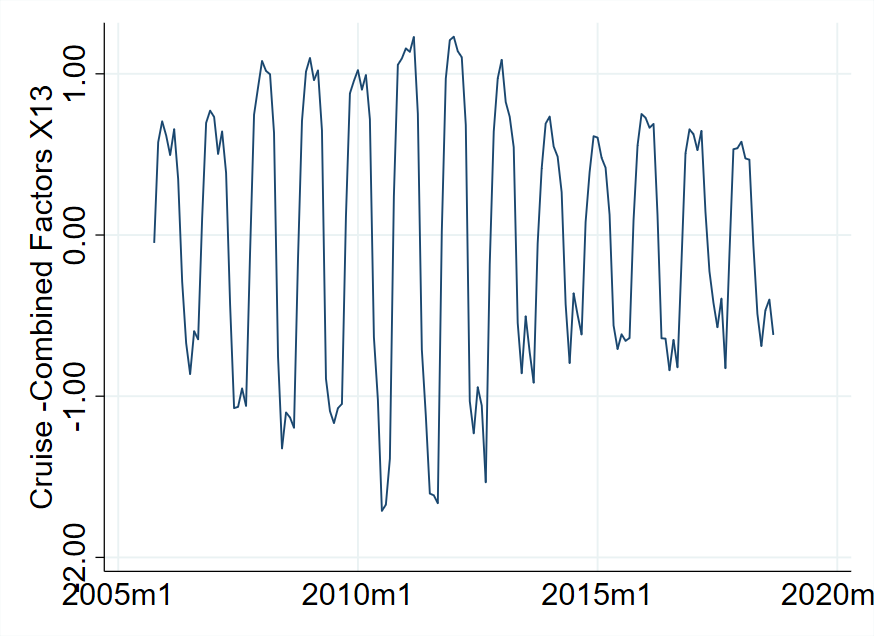
\includegraphics[width=\textwidth]{plots_1/x13_crui_1.png}
    \end{subfigure}
    \begin{subfigure}[t]{0.45\textwidth}
          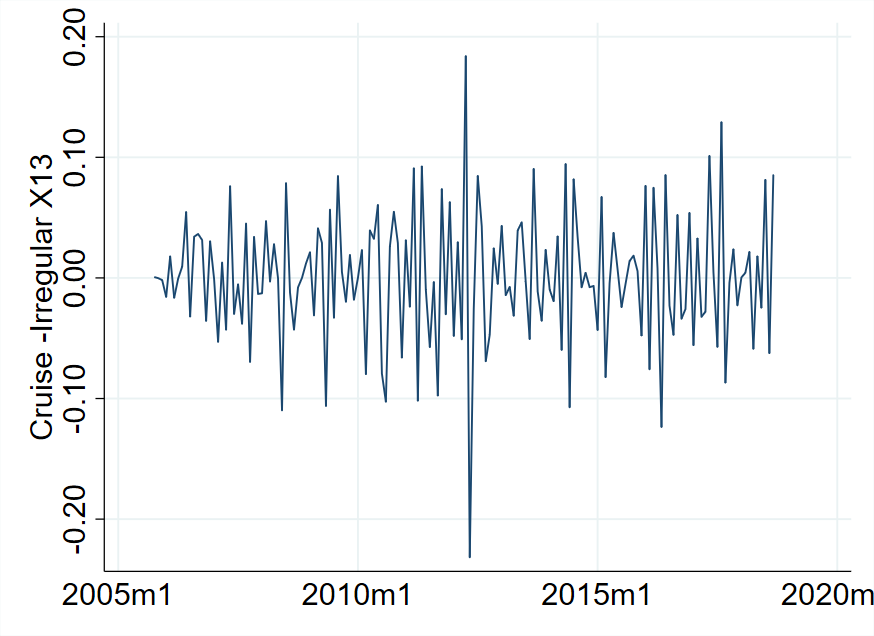
\includegraphics[width=\textwidth]{plots_1/x13_crui_2.png}
    \end{subfigure}
    \begin{subfigure}[t]{0.45\textwidth}
         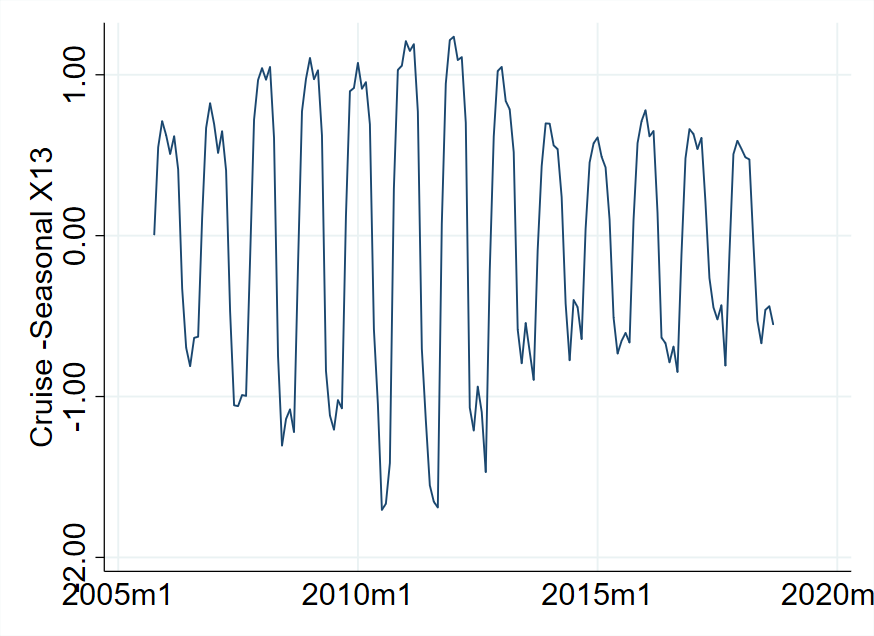
\includegraphics[width=\textwidth]{plots_1/x13_crui_3.png}
    \end{subfigure}
    \begin{subfigure}[t]{0.45\textwidth}
          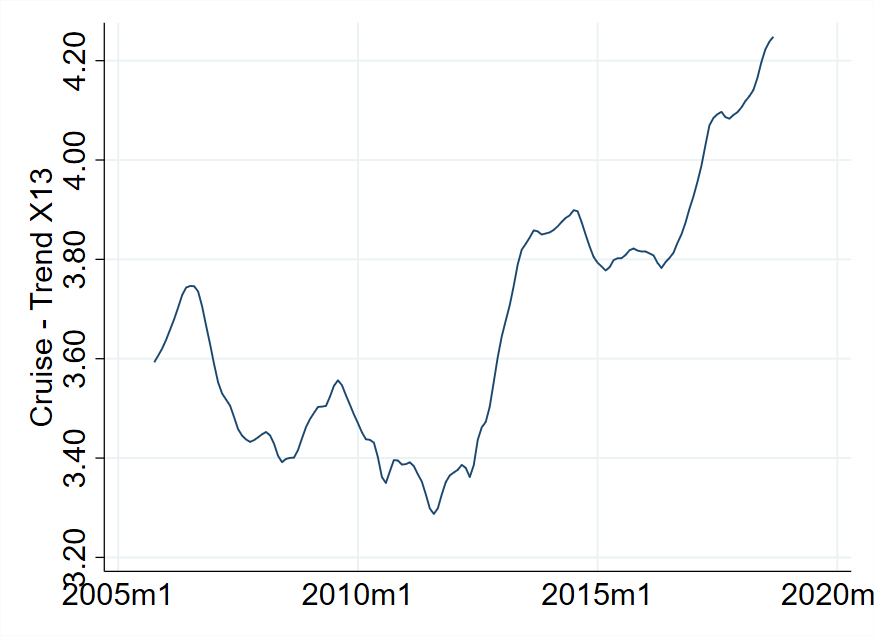
\includegraphics[width=\textwidth]{plots_1/x13_crui_4.png}
    \end{subfigure}
    \caption{Seasonal components for Cruise series using X-13 Arima Seats}
    \label{fig:x13arimacruise1}
\end{figure}

\begin{figure}[h!]
    \centering
    \begin{subfigure}[t]{0.45\textwidth}
         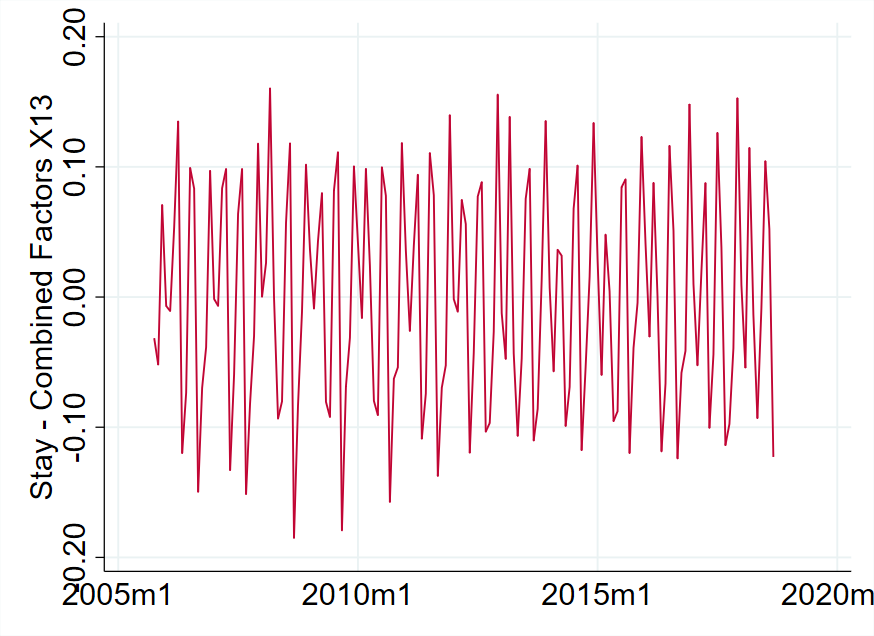
\includegraphics[width=\textwidth]{plots_1/x13_stay_1.png}
    \end{subfigure}
    \begin{subfigure}[t]{0.45\textwidth}
          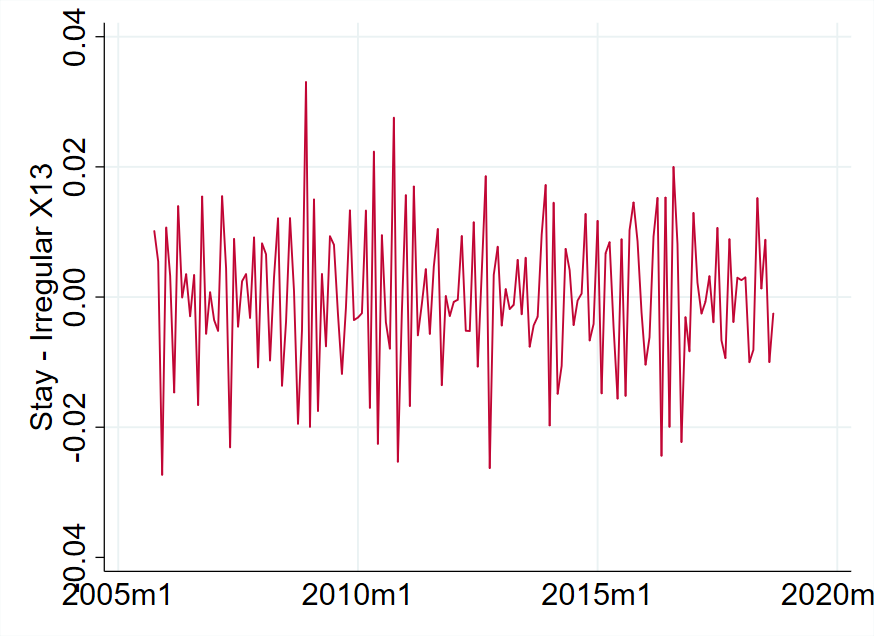
\includegraphics[width=\textwidth]{plots_1/x13_stay_2.png}
    \end{subfigure}
    \begin{subfigure}[t]{0.45\textwidth}
         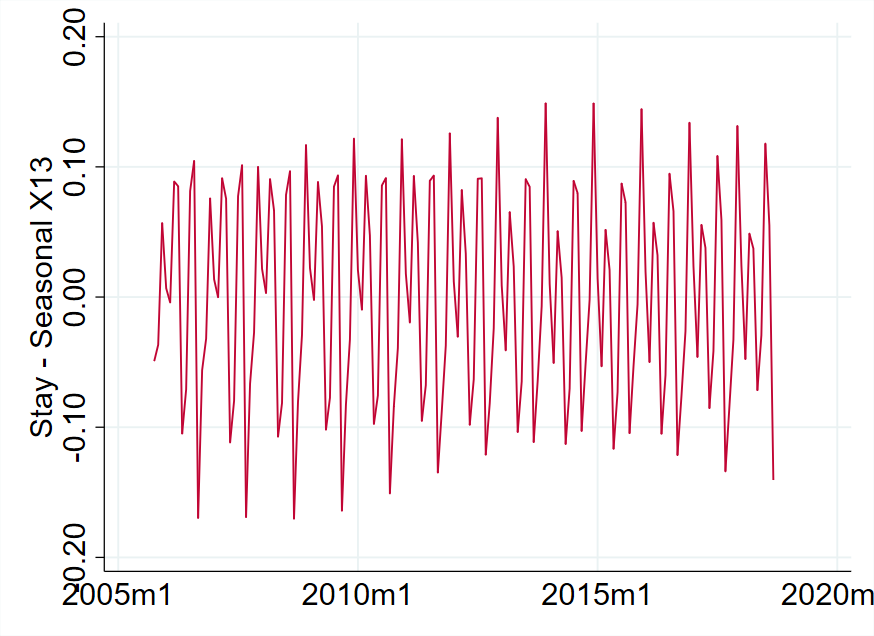
\includegraphics[width=\textwidth]{plots_1/x13_stay_3.png}
    \end{subfigure}
    \begin{subfigure}[t]{0.45\textwidth}
          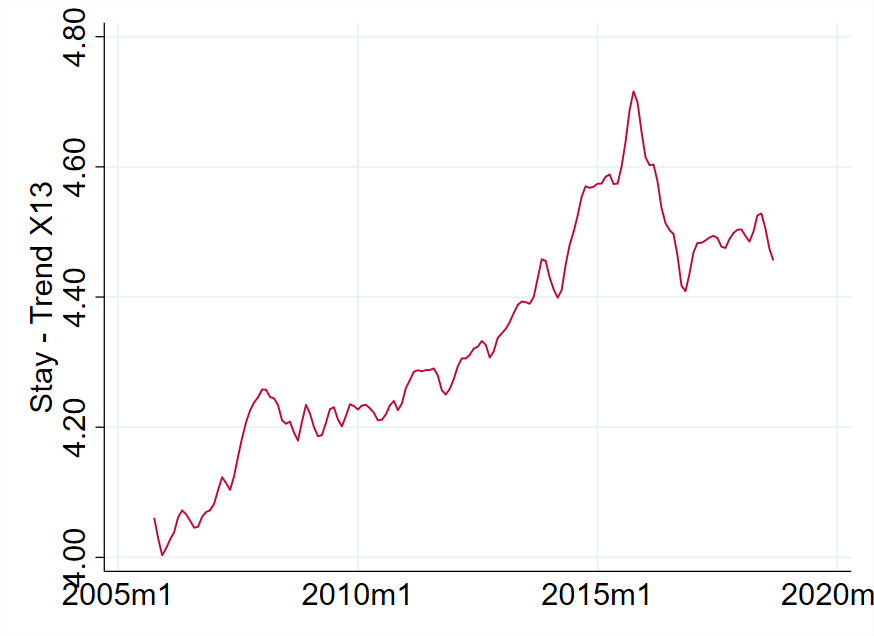
\includegraphics[width=\textwidth]{plots_1/x13_stay_4.png}
    \end{subfigure}
    \caption{Seasonal components for Stay-over series using X-13 Arima Seats}
    \label{fig:x13arimastay1}
\end{figure}


\newpage
\subsection{Compare outcomes for the seasonally adjusted series data}
The comparison is shown in the graphs in figures \ref{fig:campletx13d}

\subsection{Do the seasonal adjustment filters produce similar seasonal patterns?} 
Yes, both seasonal filters produce very similar patterns. As shown in the graphs \ref{fig:campletx13d} where series in blue represent Cruise Visitors, and series in red Stay-Over Visitors. The dashed lines are the series generated by Camplet and the solid lines are the series generated by X13 Arima Seats.\\

Some gaps can be seen in the seasonal adjustment of the Cruise Visitors series. This could be due to missing values from october, november and decemeber of 2005. I believe that it means that the Camplet algorithm is much more sensitive to gaps than X13 Arima Seats.
%	camp_vs_x13_1.png camp_vs_x13_2.png
%	camp_vs_x13_3.png camp_vs_x13_4.png

\begin{figure}[H]
    \centering
    \begin{subfigure}[t]{0.45\textwidth}
         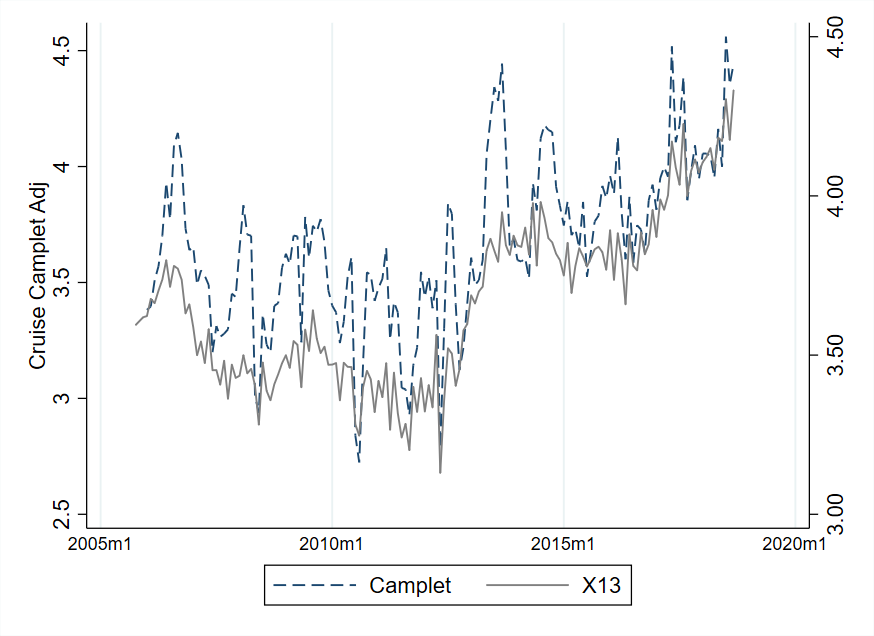
\includegraphics[width=\textwidth]{plots_1/camp_vs_x13_1.png}
    \end{subfigure}
    \begin{subfigure}[t]{0.45\textwidth}
          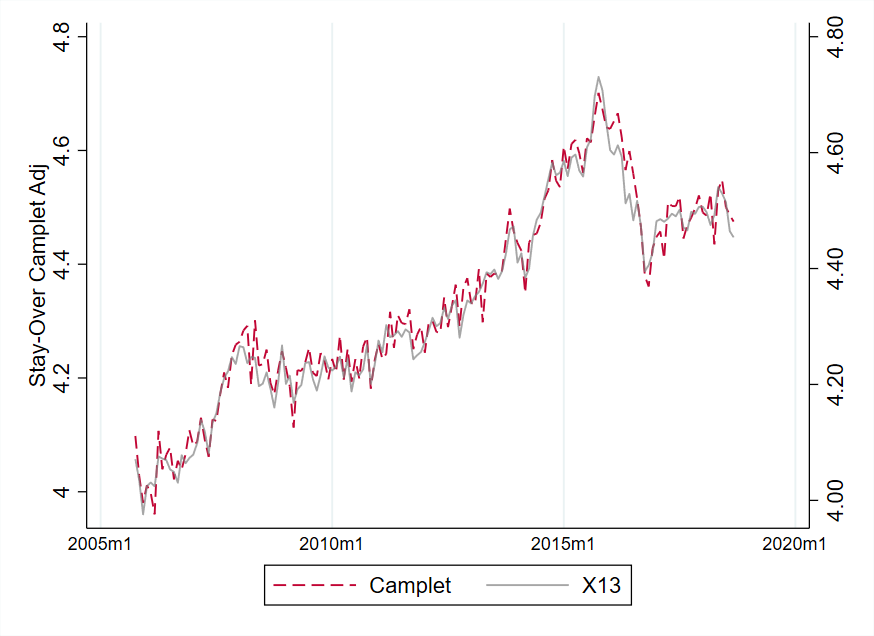
\includegraphics[width=\textwidth]{plots_1/camp_vs_x13_2.png}
    \end{subfigure}
    \begin{subfigure}[t]{0.45\textwidth}
         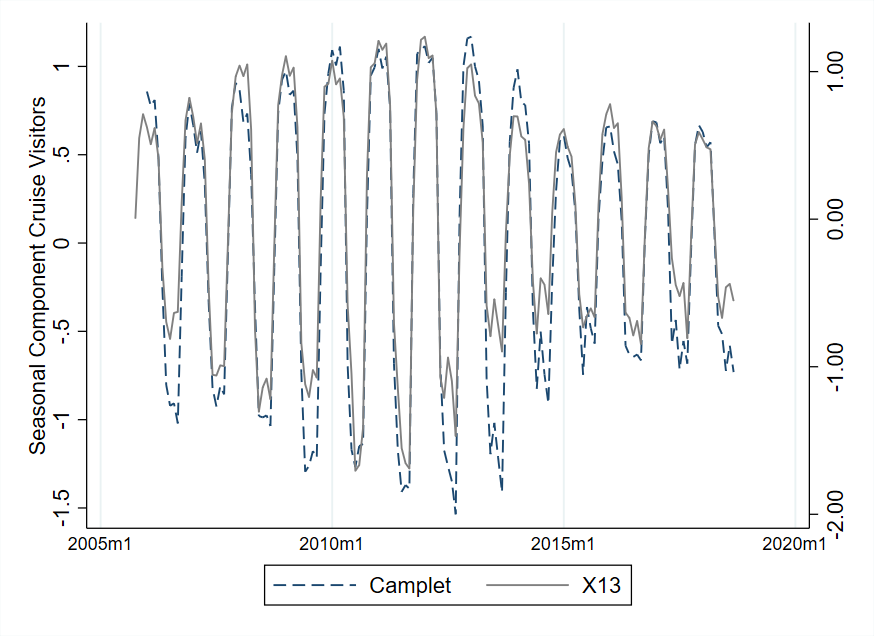
\includegraphics[width=\textwidth]{plots_1/camp_vs_x13_3.png}
    \end{subfigure}
    \begin{subfigure}[t]{0.45\textwidth}
          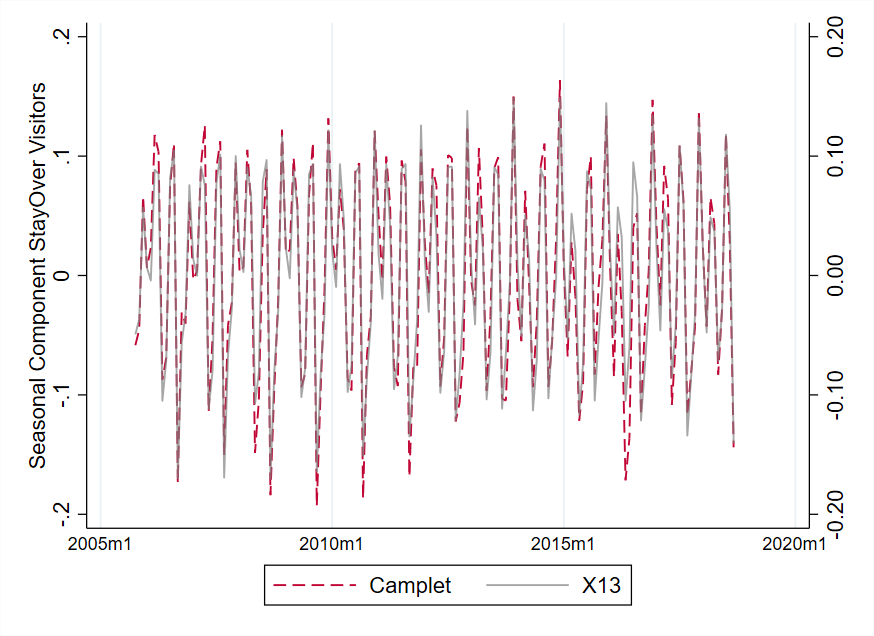
\includegraphics[width=\textwidth]{plots_1/camp_vs_x13_4.png}
    \end{subfigure}
    \caption{Comparison of the two seasonal adjustments.\label{fig:campletx13d}}
\end{figure}

\subsection{What happens if the last year of quarterly observations is discarded in the seasonal adjustment?}
% camp_vs_x13_1_b.png camp_vs_x13_2_b.png
% 	cruise_stay_camplet_1_b.png cruise_stay_x13_1_b.png
In general the adjustment does not change. Although for the cruise visitors series the gap between the two seasonal adjustment closes.

\begin{figure}[H]
    \centering
    \begin{subfigure}[t]{0.45\textwidth}
         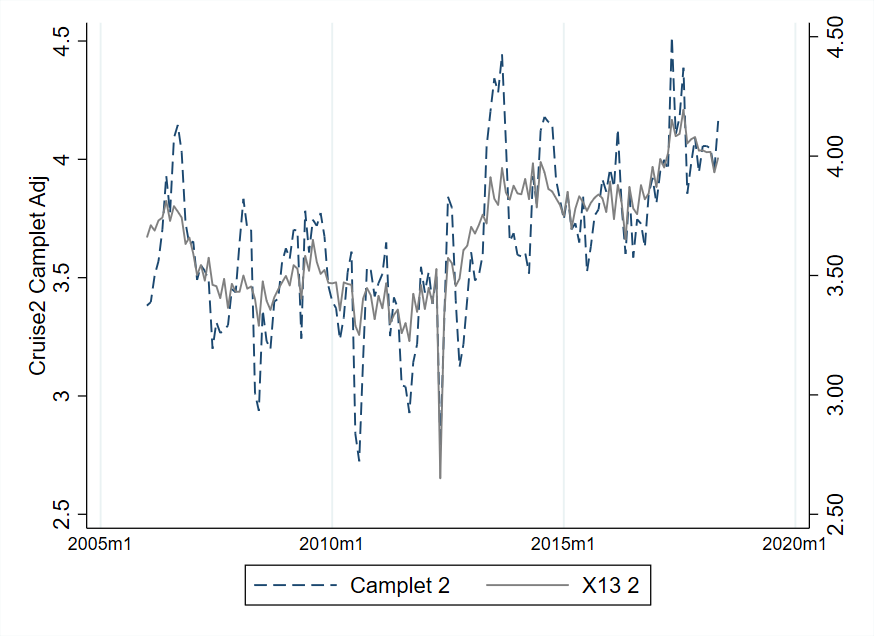
\includegraphics[width=\textwidth]{plots_1/camp_vs_x13_1_b.png}
    \end{subfigure}
    \begin{subfigure}[t]{0.45\textwidth}
          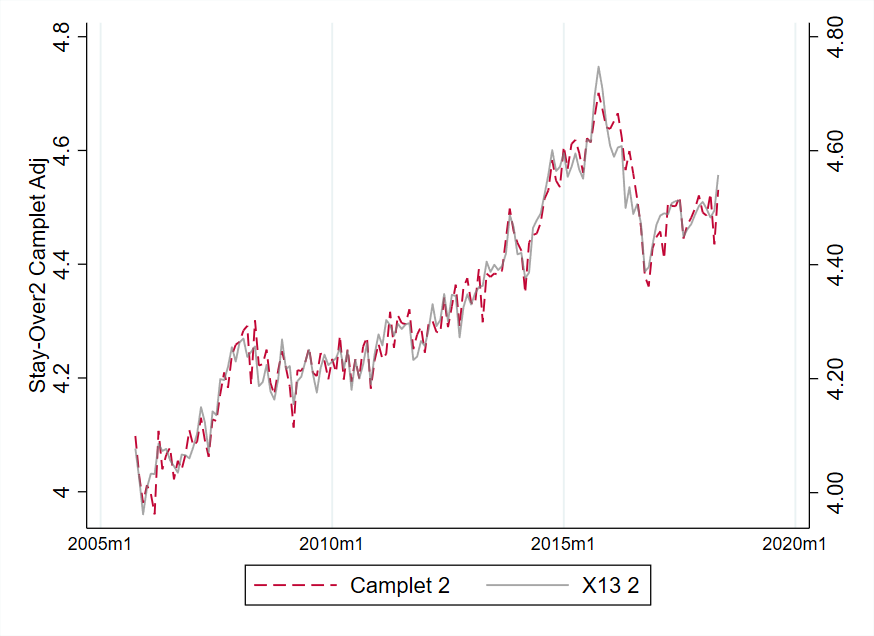
\includegraphics[width=\textwidth]{plots_1/camp_vs_x13_2_b.png}
    \end{subfigure}
    \caption{Cruise visitors vs Stay Over- without last year of quarterly observations}
    \label{fig:minus4months}
\end{figure}


\subsection{Do the seasonally adjusted data lead to changes in your modelling}
Do the seasonally adjusted data lead to changes in your modelling approach described above? Not really, the seasonally adjusted data confirms that the two series behave in correspondence to each other. The graphs \ref{fig:behaviourafteradjs} confirm that there is a common behaviour between the two series. For instance, When one of the series has particularly high values, the other exhibits the opposite- low values. This happens during 2005 and 2015. The X13 Arima Seats shows this constants more clearly. Consequently, I will consider a VAR model where both of the series are Cointegrated.

%cruise_stay_camplet_1
%cruise_stay_x13_1


\begin{figure}[h!]
    \centering
    \begin{subfigure}[t]{0.45\textwidth}
         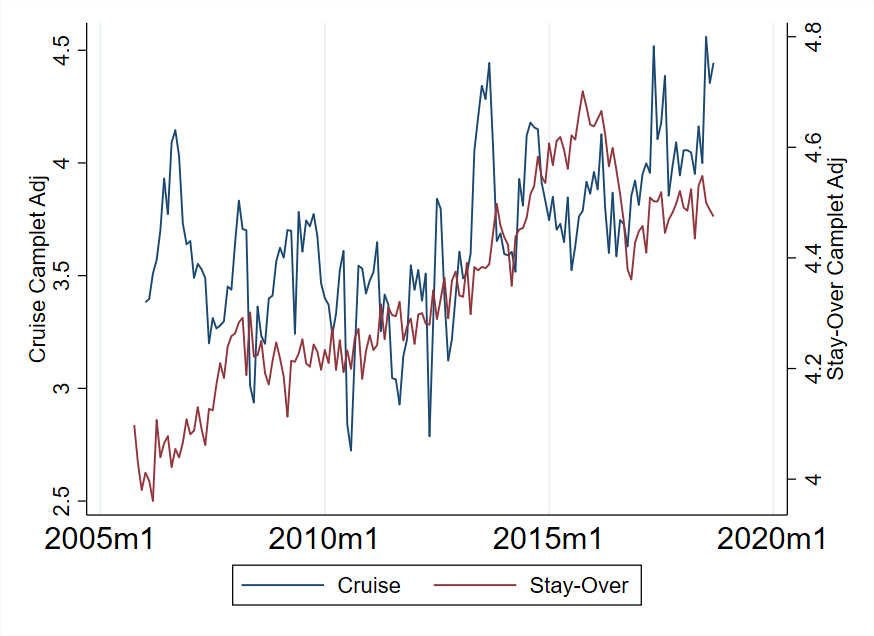
\includegraphics[width=\textwidth]{plots_1/cruise_stay_camplet_1.png}
    \end{subfigure}
    \begin{subfigure}[t]{0.45\textwidth}
          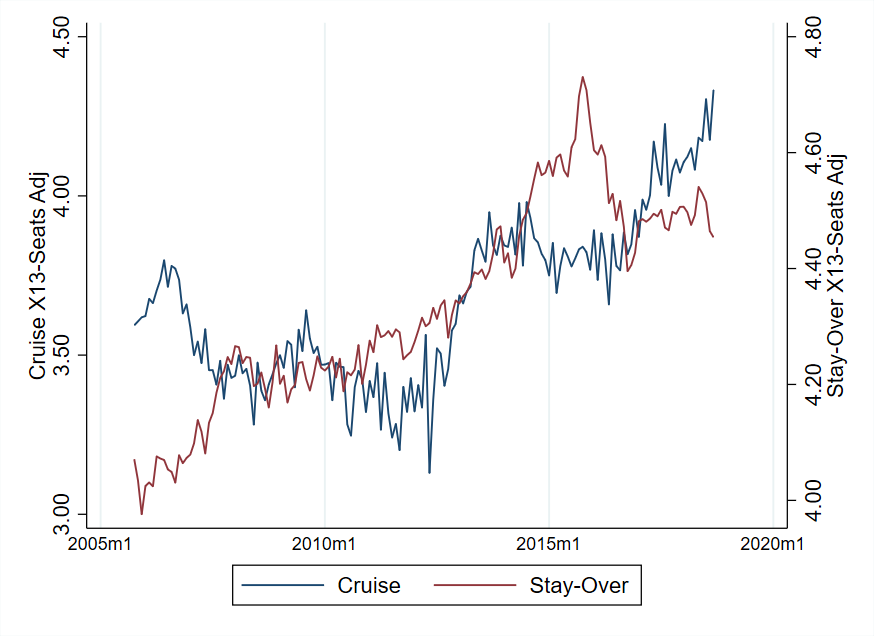
\includegraphics[width=\textwidth]{plots_1/cruise_stay_x13_1.png}
    \end{subfigure}
    \caption{Comparison two series after adjustment}
    \label{fig:behaviourafteradjs}
\end{figure}

%cruise_stay_camplet_1_c.png
	%cruise_stay_x13_1_c.png


%%%%%%%%%%%%%%%%%%%%%%%%%%%%%%%%%%%%%%%%%%%%%%%%%%%%%%%%%%%%%%%%%%%%%%%%%%%%%%%%%%%%%%
\newpage
\section{Exercise 2 Stationarity and Granger-causality}

\subsection{Unit-roots}
Test both visitors series for unitroots using ADF and KPSS test. What are your findings?\\

I use the command \textbf{dfuller} in Stata which performs the augmented Dickey-Fuller test that a variable follows a unit-root process. This command allows me to test four cases: (1) Default Unit Root as random walk without drift, (2) Random walk with trend, (3) Random walk with drift, and (4) Random walk with a constant. I represent these four cases in the following two tables. \\
In every case, the null hypothesis is that the series contains a unit root, and the alternative is that the variable was generated by a stationary process. \\
In table \ref{tab:dfuller1}, I report the Test Statistic of each regression and the MacKinnon approximate p-value for Z(t). In addition, I perform the test for the two adjusted versions of the two series.

% For 152 observations, Dickey-Fuller test for unit root presents the following critical values
% \begin{center}
% \captionof{table}{Unit Root Tests Dickey Fuller} \label{tab:dfuller1} 
%     \begin{tabular}{c|c|c|c|c}
%     \toprule
%         &   Test        & 1\% Critical	& 5 \%	Critical	& 10\%	Critical \\
%         &	Statistic   &		Value	& Value             &		Value \\
% Z(t)    &	-3.923	    &	-3.493	    &	-2.887          &		-2.577 \\
%     \bottomrule
%     \end{tabular}
% \end{center}							

%
\begin{table} \centering
\captionof{table}{Unit Root Tests Dickey Fuller} \label{tab:dfuller1} 
        \begin{tabular}{l c|c|c|c|c}
\toprule
            &   \multicolumn{2}{c}{ LN Cruise Seasonally Adj} &    \multicolumn{2}{c}{LN Stay-Over Seasonally Adj}\\
%\midrule            
            &    Camplet &  X13-Seats &     Camplet &  X13-Seats \\
            \midrule
\multirow{ 2}{*}{Unit Root} & Zt          &      -3.923&      -1.818&      -1.837&      -1.529 \\
& p           &       0.002&       0.372&       0.362&       0.519\\
\hline
\multirow{ 2}{*}{Trend} & Zt          &      -4.883&      -3.406&      -3.707&      -2.257\\
& p           &       0.000&       0.051&       0.022&       0.458\\
\hline
\multirow{ 2}{*}{Drift} & Zt          &      -3.923&      -1.818&      -1.837&      -1.529\\
& p           &       0.000&       0.036&       0.034&       0.064\\
\hline
\multirow{ 2}{*}{Constant} & Zt          &      -3.923&      -1.818&      -1.837&      -1.529\\
& p           &       0.002&       0.372&       0.362&       0.519\\
\bottomrule
\end{tabular}
\end{table}

With the seasonal adjusted series by Camplet I can reject the null hypothesis that log Cruise Visitors exhibits a unit root. However, with the seasonal adjusted series by X13 Arima Seats I cannot reject the null hypothesis that the Cruise and Stay Over series exhibit a unit root.

I then test the Integrated series of order $I(1)$ using again Dickey-Fuller test. The null hypothesis is similar. $H_0$ is that the integrated series contain a unit root, and the alternative is that the series is a stationary process. Now all the p-values indicate that it is possible to reject the null hypothesis for unit roots.  
\begin{center}
        \begin{tabular}{l c|P{2.5cm}|P{2.5cm}|P{2.5cm}|P{2.5cm}}
\toprule
            &   \multicolumn{2}{c}{$I(1)$ LN Cruise Seasonally Adj} &    \multicolumn{2}{c}{$I(1)$ LN Stay-Over Seasonally Adj}\\
 &    Camplet &  X13-Seats &     Camplet &  X13-Seats \\
\midrule 
\multirow{ 2}{*}{Unit Root} & Zt          &     -14.686&     -23.322&     -18.769&     -13.336\\
& p           &       0.000&       0.000&       0.000&       0.000\\
\hline
\multirow{ 2}{*}{Trend} & Zt          &     -14.647&     -23.443&     -18.743&     -13.355\\
& p           &       0.000&       0.000&       0.000&       0.000\\
\hline
\multirow{ 2}{*}{Drift} & Zt          &     -14.686&     -23.322&     -18.769&     -13.336\\
& p           &       0.000&       0.000&       0.000&       0.000\\
\hline
\multirow{ 2}{*}{Constant} & Zt          &     -14.686&     -23.322&     -18.769&     -13.336\\
& p           &       0.000&       0.000&       0.000&       0.000\\
\bottomrule
\end{tabular}
\end{center}

Similarly, Stata has the routine \textbf{kpss} that performs the Kwiatkowski-Phillips-Schmidt-Shin test for trend stationarity. In this test, the null hypothesis claims stationary versus an alternative hyphotesis of non-trend stationarity. According to the Stata output, the KPSS test the number of lags used for this series is a maximum of 13 chosen by Schwert criterion. It contrasts the test statistic for each lag against the critical values. Moreover, it computes autocovariances weighted by Bartlett kernel. In the table \ref{tab:kpss} I report the test statistic for the lag order 0 and lag order 13, for the log version of the adjusted series and the integrated $I(1)$ version of the series.

\begin{table} \centering
\captionof{table}{Unit Root Tests KPSS} \label{tab:kpss} 
        \begin{tabular}{l|P{2.5cm}|P{2.5cm}|P{2.5cm}|P{2.5cm}}
\toprule
            &   \multicolumn{2}{c}{Cruise Seasonally Adj} &    \multicolumn{2}{c}{Stay-Over Seasonally Adj}\\
\midrule 
LN          &            &            &            &            \\
Lag(0)      &       0.860&       2.208&       0.810&       0.903\\
Lag(13)     &       0.178&       0.219&       0.093&       0.097\\
\midrule 
D1          &            &            &            &            \\
Lag(0)      &       0.011&       0.011&       0.024&       0.048\\
Lag(13)     &       0.060&       0.049&       0.071&       0.077\\
\bottomrule
\multicolumn{5}{l}{Critical values for $H_0$: Series are trend stationary}\\
\multicolumn{5}{l}{10\%: 0.119  5\% : 0.146  2.5\%: 0.176  1\% : 0.216}
\end{tabular}
\end{table}

Once the series are differentiated I cannot reject the null $H_0$ that the two series are trend stationary. In other words, the first difference is necessary to analyze the underlying stationary process of the seasonally adjusted series of Cruise visitors and Stay-Over visitors.

%%%%%%%%%%%%%%%%%%%%%%%%%%%%%%%%%%%%%%%%%%%%%%%%%%%%%%%%%%%%%%%%%%%%%%%%%%%%%%%%%%%%%%
\subsection{Granger Causality}
Test the two seasonally adjusted visitors for Granger-causality. What do you find? Do you think this outcome is plausible? Motivate your answer. \\

To test Granger Causality I use two Stata commands. First I run a VAR regression between the seasonally adjusted series, not yet integrated. Second I use the command \textbf{vargranger}. The output of the VAR regressions below. Here I report the $chi2$ statistic and the pvalue of the Granger test. \\
The first row of table \ref{tab:granger} is a Wald test that the coefficients on the two lags of Stay-Over visitors that appear in the regression for Cruise visitors. The null hypothesis being that the coefficients are jointly zero.
The second row, is the Wald test for the coefficients on the two lags of Cruise visitors in the regression for Stay-Over.

\begin{table} \centering
\captionof{table}{Granger Causality Test} \label{tab:granger} 
        \begin{tabular}{l|P{2.5cm}|P{2.5cm}|P{2.5cm}}
\toprule
	& chi2	& df & 	p \\
\midrule	
Cruise : Stay-Over &	4.699 &	2 &	0.095 \\
%Cruise : All & 	4.699 & 	2	& 0.095 \\
\hline
Stay-Over : Cruise &	1.792 &	2	& 0.408  \\
%Stay-Over : ALL &	1.792	& 2	& 0.408 \\
\bottomrule
\end{tabular}
\end{table}

The results show that the null hypothesis that Stay-Over visitors does not Granger-cause cruise cannot be rejected. Hence, I cannot reject the hypothesis that stay-over visitors does not \textit{Granger-cause} cruise visitors. This is clear evidence that a long run steady state equilibrium exist between the two series.

For me this result makes sense because Cointegration is a property of nonstationary series, which is the case of the two series of the analysis. In addition, the time-behaviour of the series showed some trade-off between the series. Particularly, during 2005 and 2015. Moreover, from an economic perspective one can expected that the dynamics between Cruise Visitors complements the dynamics of Stay-Over visitors in the long run.

\begin{table}[htbp]\centering
\def\sym#1{\ifmmode^{#1}\else\(^{#1}\)\fi}
\caption{Regression table\label{var\_cam}}
\begin{tabular}{l*{1}{c}}
\hline\hline
                    &\multicolumn{1}{c}{(1)}\\
                    &\multicolumn{1}{c}{Adjusted Cruise Visitors}\\
\hline
Adjusted Cruise Visitors&                     \\
L.Adjusted Cruise Visitors&       0.712\sym{***}\\
                    &      (8.72)         \\
[1em]
L2.Adjusted Cruise Visitors&      0.0501         \\
                    &      (0.60)         \\
[1em]
L.Adjusted Stay-Over Visitors&       0.482         \\
                    &      (1.26)         \\
[1em]
L2.Adjusted Stay-Over Visitors&      -0.251         \\
                    &     (-0.66)         \\
[1em]
Constant            &      -0.125         \\
                    &     (-0.28)         \\
\hline
Adjusted Stay-Over Visitors&                     \\
L.Adjusted Cruise Visitors&      0.0180         \\
                    &      (1.13)         \\
[1em]
L2.Adjusted Cruise Visitors&    -0.00529         \\
                    &     (-0.33)         \\
[1em]
L.Adjusted Stay-Over Visitors&       0.569\sym{***}\\
                    &      (7.59)         \\
[1em]
L2.Adjusted Stay-Over Visitors&       0.381\sym{***}\\
                    &      (5.16)         \\
[1em]
Constant            &       0.174\sym{*}  \\
                    &      (1.99)         \\
\hline
Observations        &         151         \\
\hline\hline
\multicolumn{2}{l}{\footnotesize \textit{t} statistics in parentheses}\\
\multicolumn{2}{l}{\footnotesize \sym{*} \(p<0.05\), \sym{**} \(p<0.01\), \sym{***} \(p<0.001\)}\\
\end{tabular}
\end{table}

\begin{table}[htbp]\centering
\def\sym#1{\ifmmode^{#1}\else\(^{#1}\)\fi}
\caption{Regression table\label{var\_x13}}
\begin{tabular}{l*{1}{c}}
\hline\hline
                    &\multicolumn{1}{c}{(1)}\\
                    &\multicolumn{1}{c}{Final SEATS Seasonal Adjustment Component}\\
\hline
Final SEATS Seasonal Adjustment Component&                     \\
L.Final SEATS Seasonal Adjustment Component&       0.412\sym{***}\\
                    &      (6.01)         \\
[1em]
L2.Final SEATS Seasonal Adjustment Component&       0.556\sym{***}\\
                    &      (8.05)         \\
[1em]
L.Final SEATS Seasonal Adjustment Component&       0.159         \\
                    &      (0.72)         \\
[1em]
L2.Final SEATS Seasonal Adjustment Component&     -0.0984         \\
                    &     (-0.44)         \\
[1em]
Constant            &      -0.142         \\
                    &     (-0.83)         \\
\hline
Final SEATS Seasonal Adjustment Component&                     \\
L.Final SEATS Seasonal Adjustment Component&     -0.0132         \\
                    &     (-0.54)         \\
[1em]
L2.Final SEATS Seasonal Adjustment Component&      0.0234         \\
                    &      (0.95)         \\
[1em]
L.Final SEATS Seasonal Adjustment Component&       0.908\sym{***}\\
                    &     (11.40)         \\
[1em]
L2.Final SEATS Seasonal Adjustment Component&      0.0591         \\
                    &      (0.75)         \\
[1em]
Constant            &       0.107         \\
                    &      (1.74)         \\
\hline
Observations        &         154         \\
\hline\hline
\multicolumn{2}{l}{\footnotesize \textit{t} statistics in parentheses}\\
\multicolumn{2}{l}{\footnotesize \sym{*} \(p<0.05\), \sym{**} \(p<0.01\), \sym{***} \(p<0.001\)}\\
\end{tabular}
\end{table}

\begin{table}[htbp]\centering
\def\sym#1{\ifmmode^{#1}\else\(^{#1}\)\fi}
\caption{Regression table\label{granger}}
\begin{tabular}{l*{1}{c}}
\hline\hline
                    &\multicolumn{1}{c}{(1)}\\
                    &\multicolumn{1}{c}{Adjusted Cruise Visitors}\\
\hline
Adjusted Cruise Visitors&                     \\
L.Adjusted Cruise Visitors&       0.712\sym{***}\\
                    &      (8.72)         \\
[1em]
L2.Adjusted Cruise Visitors&      0.0501         \\
                    &      (0.60)         \\
[1em]
L.Adjusted Stay-Over Visitors&       0.482         \\
                    &      (1.26)         \\
[1em]
L2.Adjusted Stay-Over Visitors&      -0.251         \\
                    &     (-0.66)         \\
[1em]
Constant            &      -0.125         \\
                    &     (-0.28)         \\
\hline
Adjusted Stay-Over Visitors&                     \\
L.Adjusted Cruise Visitors&      0.0180         \\
                    &      (1.13)         \\
[1em]
L2.Adjusted Cruise Visitors&    -0.00529         \\
                    &     (-0.33)         \\
[1em]
L.Adjusted Stay-Over Visitors&       0.569\sym{***}\\
                    &      (7.59)         \\
[1em]
L2.Adjusted Stay-Over Visitors&       0.381\sym{***}\\
                    &      (5.16)         \\
[1em]
Constant            &       0.174\sym{*}  \\
                    &      (1.99)         \\
\hline
Observations        &         151         \\
\hline\hline
\multicolumn{2}{l}{\footnotesize \textit{t} statistics in parentheses}\\
\multicolumn{2}{l}{\footnotesize \sym{*} \(p<0.05\), \sym{**} \(p<0.01\), \sym{***} \(p<0.001\)}\\
\end{tabular}
\end{table}




%%%%%%%%%%%%%%%%%%%%%%%%%%%%%%%%%%%%%%%%%%%%%%%%%%%%%%%%%%%%%%%%%%%%%%%%%%%%%%%%%%%%%%
\newpage
\section{Exercise 3 VAR and VECM}

Columns 2-5 and 6-9 of Table 1 show two types of impulse responses with standard deviation between brackets of the VAR model of the logs of seasonally adjusted series, with a constant and a trend and three lags.

\subsection{Ortogonalized and generalized Impulse Responses}
Which columns give orthogonalized IRs (OIRs) and which generalized IRs? What is the ordering used in the OIRs? Can you comment on the plausibility of this assumption?. \\

Since it is known that Generalized Impulse Responses coincides with Orthogonalized Impulse Responses for the most endogenous variable in the VAR, and the table provided I hardly see a difference between the two columns, I conclude that the two variables and their shocks are likely correlated. Hence in this VAR model there is no ordering of the variables. It cannot be said that there is a more exogenous or endogeneous variable than the other.\\
I believe that this makes sense in the case of the tourism series because both may depend on similar economic factors and are affected by similar shocks. Perhaps further variables should be included in the model.


\subsection{VAR}
Rewrite a vector autoregressive (VAR) system with three lags in zt, which consists of two variables, as a Vector Error Correction Model.

Let's say that the VAR(3) is

\begin{align*}
 z_{t} & = \Phi_1 z_{t-1} + \Phi_2 z_{t-2} +\Phi_3 z_{t-3} + u_t \\
  & \text{where} \; z_t \; \text{is a 2 dimensional vector: Cruise and Stay Over} \\
 &  \Phi_i \; i=1,2,3 \; 2\times 2 \; \text{matrices of fixed coefficients}\\
  &  u_t \; \text{is a mean zero serially uncorrelated vector of disturbances} \\
\text{In matrix notation} & \\
  & \mathbf{z}_t=\mathbf{A(L)} \mathbf{z}_t + \mathbf{e}_t \; , \qquad
 \mathbf{e}_t ~ \; (0, \mathbf{\Omega})  \\
 & \text{where} \; \mathbf{A(L)} \text{is degree} \; 3 \\
 \text{VECM representation} & \\
 & \mathbf{A}*(L)\Delta \mathbf{z}_t = - \Pi \mathbf{z}_{t-1} + \mathbf{e}_t\\
 & \Pi = \mathbf{A}(3) \; \text{degree of} \; \mathbf{A}*(L)=(3-1)=2
 \end{align*}
 

\subsection{VEC}
What are the possible outcomes and implications for the rank of the parameter matrix of $z_{t-1}$ in the Vector Error Correction Model?\\

The $rank(\Pi)$ can be between $0$ and $m=2$. Therefore, in this case the possible outcomes for the rank
\begin{align*}
    \text{Rank}\Pi = r < 2 \; \therefore \; 1
\end{align*}
The implication of the rank defines the dimension of the cointegration space
\begin{align*}
    & r= 0 \; : \; \text{nonstationary variables, no cointegration, VAR in first differences} \\
    & r=2 \; : \; \text{stationary variables; VAR in levels}
\end{align*}

\subsection{Graphs and Impulse response: long-run cointegratng}
Do the graphs of the series and the impulse responses in Table 1 suggest
the existence of a long-run cointegrating relation between cruise visitors
and stay-over visitors (both seasonally adjusted and in logs)? \\

Yes, both the graphs and the Impulse Responses Coefficients suggest that the series are cointegrated. However, it is necessary to seasonally adjust the series. As I discussed in the previous two exercises.

\subsection{Cointegration test}

Carry out a co-integration test. What do you find? \\

In Stata I run the command \textbf{vecrank} which performs the Johansen test for cointegration. According to the test, the trace statistic at $r=0$ of 4.84 is less than its critical value of 15.41, I cannot reject the null hyphotesis that the two series in the system are part of a cointegrated equation. 

%\begin{center}
\begin{table}[H] \centering
\caption{Johnasen Cointegration Test\label{johnasen}}
\begin{tabular}{llllll}
\toprule
rank & parms & LL        & eigenvalue & statistic & value \\
\midrule
0    & 6     & 482.9493  & .          & 4.8402*   & 15.41 \\
1    & 9     & 485.2964  & 0.03002    & 0.1460    & 3.76  \\
2    & 10    & 485.36942 & 0.00095    &           &      \\
\bottomrule
\end{tabular}
\end{table}
This result confirms the finding of the Granger test and the previous discussion.
%\end{center}



%%%%%%%%%%%%%%%%%%%%%%%%%%%%%%%%%%%%%%%%%%%%%%%%%%%%%%%%%%%%%%%%%%%%%%%%%%%%%%%%%%%%%%

\newpage
\section{Exercise 4. State Space forms}



\begin{itemize}
    \item Write $VAR(2)$ and $MA(2)$ and $ARMA(2,2)$ processes in state-space form SSF
\end{itemize}
    
%I have to download the seasonally adjusted US real GDP series
%https://research.stlouisfed.org/useraccount/apikey
%https://www.stata.com/manuals/dimportfred.pdf
% First, I start by describing the a ARMA(2,2)
% \begin{align*}
%     y_t =& \mathbf{x}_t\beta + \rho_1(y_{t-1} - \mathbf{x}_{t-1}) +\rho(y_{t-2} - \mathbf{x}_{t-2} \beta) + \theta_1\epsilon_{t-1} + \theta_2\epsilon_{t-2}  +\epsilon \\
%     \rho &\; \text{first order autocorrelation parameter} \\
%     \theta & \; \text{first order moving average parameter} \\
%     \epsilon_t & \; ~ i.i.d. \; N(0,\sigma^2) 
% \end{align*}

% I can now write the $VAR(2)$ in state space form as follows:

% \begin{align*}
%     \mathbf{y}_t & = \mathbf{A_1} \mathbf{Y}_{t-1} + \mathbf{A_2} \mathbf{Y}_{t-2} +\mathbf{B}_0 \mathbf{x}_t +\mathbf{u}_t \\
%   & \mathbf{y}_t  : \; K \times 1 \; \text{vector of endogenous variables} \\
%     & \mathbf{A}  : \; K \times K2 \; \text{matrix of coefficients} \\
%     & \mathbf{B}_0  : \; K \times M \; \text{matrix of coefficients} \\
%     & \mathbf{x}_t  : \; M \times 1 \; \text{vector of exogenous variables} \\
%     & \mathbf{u}_t  : \; K \times 1 \; \text{vector of white noise innovations}
% \end{align*}
\subsection{VAR(2)}
 \begin{align*}
    y_t =& \mathbf{x}_t\beta + \rho_1(y_{t-1} - \mathbf{x}_{t-1} \beta) +\rho(y_{t-2} - \mathbf{x}_{t-2} \beta) +\epsilon \\
    \rho &\; \text{first order autocorrelation parameter} \\
    \epsilon_t & \; ~ i.i.d. \; N(0,\sigma^2) 
\end{align*}
I define the system equation as
\begin{align*}
    \text{System equation}: \qquad \mathbf{z}_t & = \mathbf{A} \mathbf{z}_{t-1}+ \mathbf{B} \epsilon_t \\
    \text{Observed equation}: \qquad \mathbf{y}_t & = \mathbf{C} \mathbf{z}_t \\
& \mathbf{z}_t = \begin{bmatrix}
    Y_t & Y_{t-1}  & Y_{t-2} \\
    \mathbf{x}_t & \mathbf{x}_{t-1}  & \mathbf{x}_{t-2} 
\end{bmatrix}
\end{align*}

\begin{align*}
    \begin{bmatrix}
   y_t\\
     y_{t-1}
\end{bmatrix}	 = 
\begin{bmatrix}
    \rho_1 & \rho_2 & \beta & \rho_1 \beta & \rho_2 \beta \\
    1 & 0 & 0 & 1 & 0 
\end{bmatrix} 
\begin{bmatrix}
    y_{t-1} \\
    y_{t-2} \\
    \mathbf{x}_t \\
    \mathbf{x}_{t-1} \\
    \mathbf{x}_{t-2} \\
\end{bmatrix} +
\begin{bmatrix}
    1 \\
    0 \\
    0 \\
    0 \\
    0
\end{bmatrix}
\epsilon
\end{align*}

\subsection{MA(2)}

 \begin{align*}
    y_t =& \mu_t  \\
    \mu_t =& \epsilon_t  +\theta_1\epsilon_{t-1} + \theta_2\epsilon_{t-2} \\
     \theta & \; \text{moving average parameter} \\
    \epsilon_t & \; ~ i.i.d. \; N(0,\sigma^2) 
\end{align*}
The space state form can be represented as follows

\begin{align*}
    \text{System equation}: \qquad \mathbf{z}_t & = \mathbf{A} \mathbf{z}_{t-1}+ \theta \epsilon_t \\
    \text{Observed equation}: \qquad \mathbf{y}_t & = \mathbf{C} \mathbf{z}_t \\
        y_t & = 
    \begin{bmatrix}
     1 & 0 & 0 
\end{bmatrix}
\mathbf{z}_t +  
\mu \\
\mathbf{z}_t & = \begin{bmatrix}
 0 & 1 & 1\\
 0 & 0 & 0
\end{bmatrix}
\mathbf{z}_{t-1} + \begin{bmatrix}
 1 \\
 \theta_1 \\
 \theta_2 
\end{bmatrix} \epsilon_t
\end{align*}

\subsection{ARMA(2,2)}

 \begin{align*}
    y_t = & \rho_1(y_{t-1}  +\rho_2(y_{t-2} +\epsilon_t + \theta_1 \epsilon_{t-1} + \theta_1 \epsilon_{t-2} \\
    \rho &\; \text{autocorrelation parameter} \\
    \theta & \; \text{moving average parameter} \\
    \epsilon_t & \; ~ i.i.d. \; N(0,\sigma^2) \\
    \text{Let} \; m=\max(p,q+1)=3 \\
y_t = & \rho y_{t-1} + \rho_2 y_{t-2} + \rho_2 y_{t-3}+\epsilon_t + \theta_1 \epsilon_{t-1} + \theta_2 \epsilon_{t-4} \\
    \text{System equation}: \qquad \mathbf{z}_t & = \mathbf{A} \mathbf{z}_{t-1}+ \mathbf{\theta} \epsilon_t \\
    \text{Observed equation}: \qquad \mathbf{y}_t & = \mathbf{C} \mathbf{z}_t \\
& \mathbf{z}_t = \begin{bmatrix}
    Y_t  \\
    \rho_2 y_{t-1} + \theta_1 \epsilon_{t} + \theta_2 \epsilon_{t-4} \\
    \rho_3 y_{t-1} + \theta_3 \epsilon_{t}
\end{bmatrix} \\
y_t = & \begin{bmatrix}
 1 & \mathbf{0}_{m-1}
\end{bmatrix} \mathbf{z}_t \\
 & \mathbf{z}_t = \begin{bmatrix}
 \rho_1 & 1 & 0 & 0 \\
 \rho_2 & 0 & 1 & 0 \\
 \rho_3 & 0 & 0 & 0 \\
\end{bmatrix} \mathbf{z}_{t-1} +
\begin{bmatrix}
 1 \\
 \theta_1 \\
 \theta_2  
\end{bmatrix} \epsilon_t
\end{align*}

\newpage
\subsection{Beveridge-Nelson}

\begin{itemize}
\item Download the seasonally adjusted US real GDP series

I use Stata 16 and its module to import data from the Federal Reserve Economic Data\footnote{Link to \href{https://www.stata.com/features/overview/import-fred/}{\textit{ St. Louis Federal Reserve}}}. To estimate the Beveridge-Nelson decomposition model I computed the components step by step in Stata and following the post in the website of Eviews (since I do not have access to this software)\footnote{\href{http://blog.eviews.com/2020/02/beveridge-nelson-filter.html}{blog.eviews.com}}. I present the code I used in the appendix. 

\begin{verbatim}
fredsearch real gross national product, tags(usa)  

import fred GDPC1 GDPPOT, daterange(1990-01-01 2019-12-31) clear
\end{verbatim}
    \item Estimate a Beveridge-Nelson trend-cycle decomposition model, assuming a unit root plus drift for the trend $\tau_t$, an $AR(2)$ process for the cycle $c_t$, and uncorrelated innovations $\eta_t, v_t$.
\end{itemize}
      
The Beveridge-Nelson decomposition determines a trend process that I called $\hat{\tau}$ and a cycle process $c_t$, such that $y_t= \tau_t+c_t$. As required, I also add a drift and assume that there is unit root (e.g I use the first difference of the log)

\begin{align*}
    y_{t} = \mu + \phi_1 y_{t-1} +\rho_2 y_{t-2} + \epsilon
\end{align*}

The first step is to fit an $AR(2)$ model, for which I assume unit root\footnote{I do not test for this}. After this I estimate and store the deterministic drift as $\hat{\mu} = \frac{\hat{\alpha}}{1-\hat{\phi}} $. Then I compute the Beveridge-Nelson cycle component \\
\begin{align*}
    \hat{\tau}_t =\Big(  y_{t} + \frac{\hat{\phi}}{1-\hat{\phi}} \Delta y_t \Big) - \Big( \frac{\hat{\phi}}{1- \hat{\phi}}\Big) \hat{\mu}
\end{align*}

Finally, I compute the Beveridge-Nelson $\hat{c}_t = y_t -  \hat{\tau}_t$

\begin{figure}[H]
    \centering
     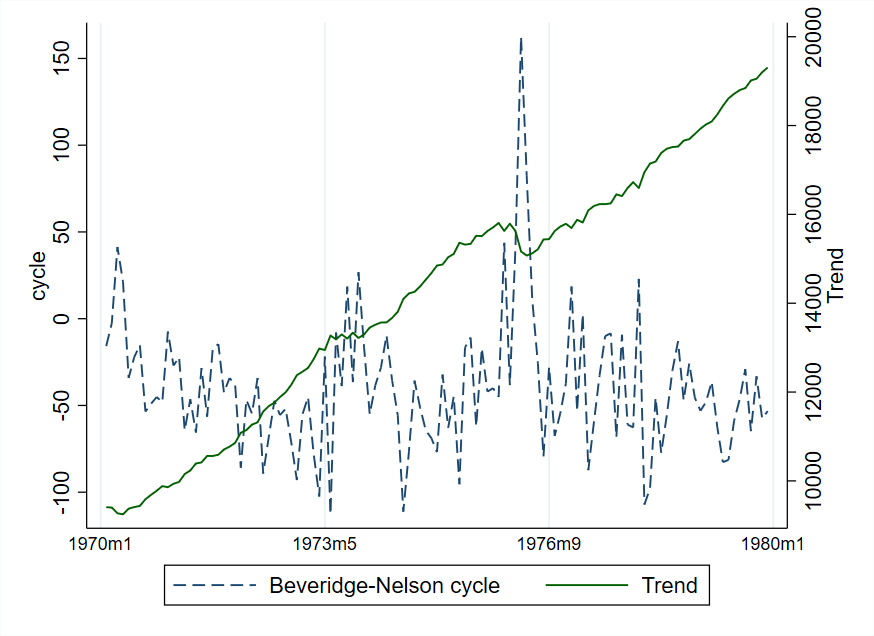
\includegraphics[width=0.6\textwidth]{plots_1/bn_cycletrend.png}
     \caption{Beveridge-Nelson: Cycle and trend}
    \label{fig:bntrend}
\end{figure}

In addition, I contrast the result of the decomposition with the GDP gap in the graph \ref{fig:bndecomp}.

\begin{figure}[H]
    \centering
     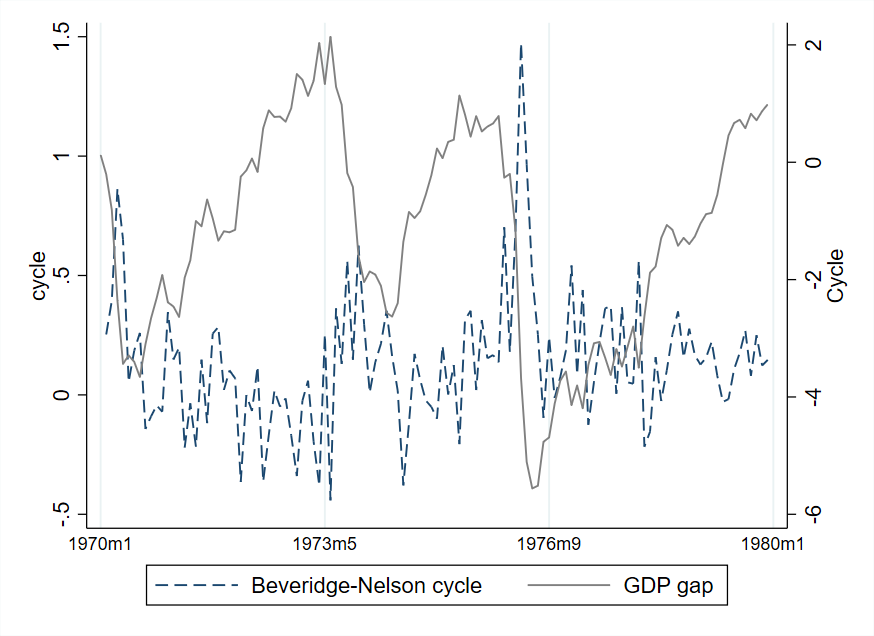
\includegraphics[width=0.6\textwidth]{plots_1/bn_decompostion.png}
     \caption{Beveridge-Nelson Cycle and  GDP gap}
    \label{fig:bndecomp}
\end{figure}

To the sake of completeness, I compare my calculation with the estimation of the in-built routine of Stata for the Hodrick-Prescott.

\begin{figure}[H]
    \centering
     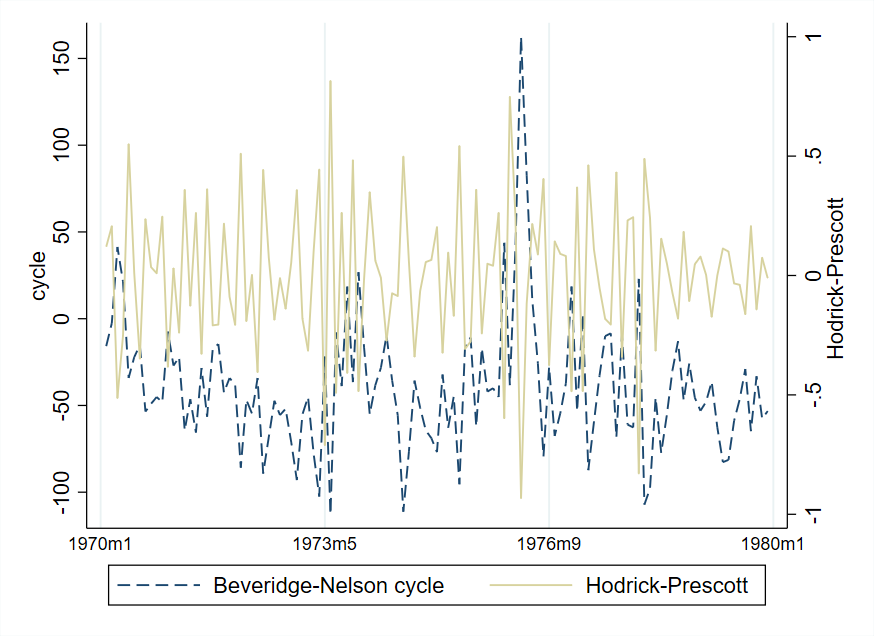
\includegraphics[width=0.6\textwidth]{plots_1/bn_hp_decom.png}
     \caption{Hodrick Prescott}
    \label{fig:bndecomps}
\end{figure}



\newpage

\section{Appendix}
\subsection{X13-ARIMA Seats}
I used the software directly downloaded from the United States Census Bureau \textit{X-13ARIMA-SEATS program (Version 1.1 Build 39) }. For each of the series I converted it first to .dat file. Then I created a spec file. These files have three purposes: (1) to establish the span of time analyzed, (2) to establish the time of adjustment e.g. Seats, and (3) to provide additional requirements e.g. compute or not the logs. The following is an example of the one of the spec files.
\begin{minted}{spec}
series{ 
    file = "ln_cruisevisitors.dat"
    period = 12
    format = Datevalue
}
transform{ 
    function = none
}
regression{ 
    variables = ( const td1coef )
    #aictest = ( td easter )
    #savelog = aictest
}
outlier{ 
    types = ( AO LS )
}
arima{ 
    model =  (1 0 0)(1 1 1)
}
forecast{ 
    maxlead = 12
    print = none
}
estimate{ 
    print = (roots regcmatrix acm)
    savelog = (aicc aic bic hq afc)
}
check{ 
    print = all
    savelog = (lbq nrm)
}
seats{ }
slidingspans{ 
    savelog = percent
    additivesa = percent}
history{ 
    estimates = (fcst aic sadj sadjchng trend trendchng)
    savelog = (asa ach atr atc)}
\end{minted}

\newpage 
\subsection{Other graphs}

\begin{figure}[H]
    \centering
        \begin{subfigure}[t]{0.45\textwidth}
         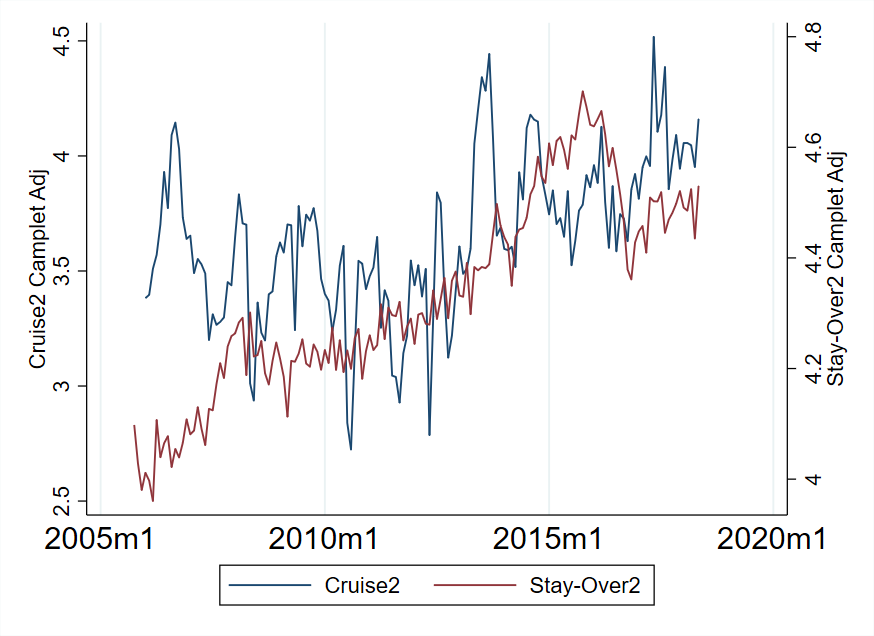
\includegraphics[width=\textwidth]{plots_1/cruise_stay_camplet_1_b.png}
    \end{subfigure}
    \begin{subfigure}[t]{0.45\textwidth}
          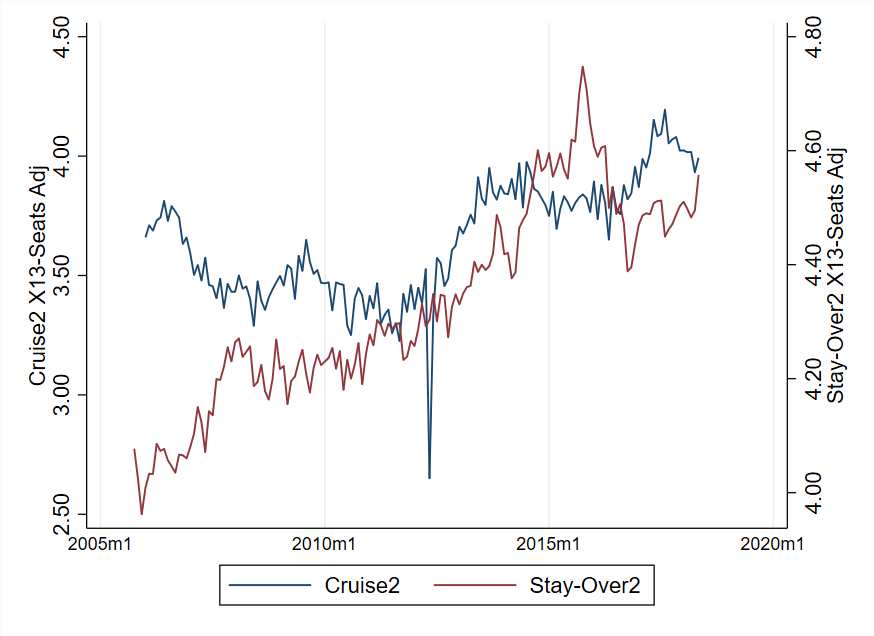
\includegraphics[width=\textwidth]{plots_1/cruise_stay_x13_1_b.png}
    \end{subfigure}
    \caption{Comparison two series after adjustment without the last year quarterly observations}
\end{figure}

\begin{figure}[H]
    \centering
    \begin{subfigure}[t]{0.45\textwidth}
         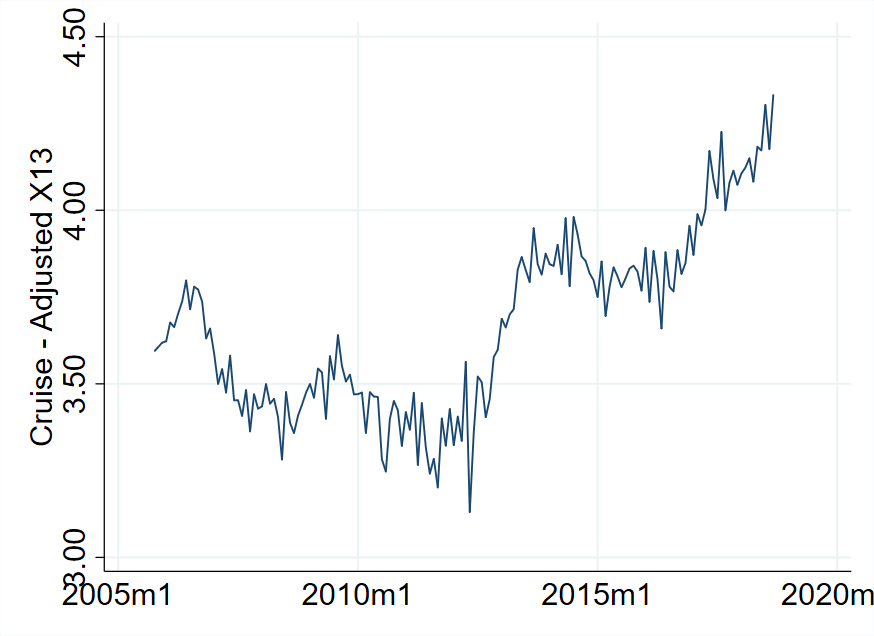
\includegraphics[width=\textwidth]{plots_1/x13_crui_5.png}
    \end{subfigure}
    \begin{subfigure}[t]{0.45\textwidth}
          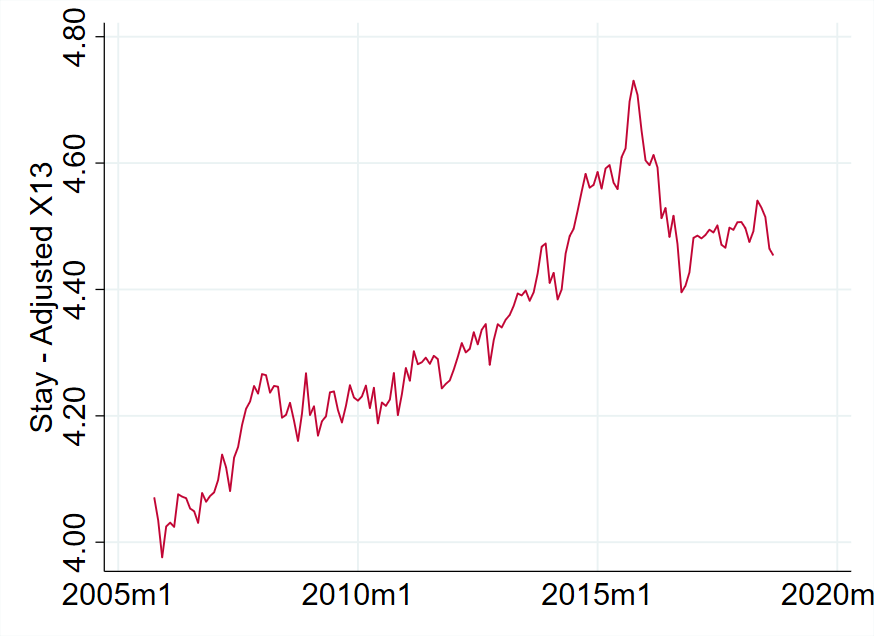
\includegraphics[width=\textwidth]{plots_1/x13_stay_5.png}
    \end{subfigure}
    \caption{Series Tourism Aruba 2005-2018}
    \label{fig:comparison}
\end{figure}

\newpage 
\subsection{Code Beveridge-Nelson Cycle}
%\begin{verbatim}
\begin{minted}{stata}
//
*Drift: errors that accumulate over time
*assuming a unit root plus drift
//
arima d_loggdp , ar(2)
	ereturn list
// Paramaters used to calculate cycle and trend
scalar alpha_hat = e(b)[1,1]
scalar phi_hat = e(b)[1,2]
scalar mu_hat = alpha_hat/(1-phi_hat)

// Trend = tau
gen tau_hat = (gdp+(phi_hat/(1- phi_hat)*d_loggdp))-(phi_hat/(1-phi_hat))*mu_hat

// Cycle 
gen cycle = gdp-tau_hat

// Plots
// The cylce and the gap
tw (tsline cycle , yaxis(1) lcolor(navy)  lpattern(dash) ///
legend(label(1 "Beveridge-Nelson cycle ")) )  ///
(tsline cbogap , yaxis(2)   ytitle("Cycle", axis(2)) ///
lcolor(gray) graphregion(color(white)) ///
plotregion( color(white)) xtitle("")  xlabel(, noticks ///
format(\%tm) labsize(small) grid) legend(label(2 "GDP gap")) 

// The cylce and the trend
tw (tsline cycle , yaxis(1) lcolor(navy)  lpattern(dash) ///
legend(label(1 "Beveridge-Nelson cycle ")) )  ///
(tsline tau_hat , yaxis(2)   ytitle("Trend", axis(2)) ///
lcolor(dkgreen) graphregion(color(white)) ///
plotregion( color(white)) xtitle("")  xlabel(, noticks format(\%tm) ///
labsize(small) grid) legend(label(2 "Trend")) 

// Comparing wiht Hodrick-Prescott 

tsfilter hp hp_vars=d_loggdp, smooth(1)

tw (tsline cycle , yaxis(1) lcolor(navy)  lpattern(dash) ///
legend(label(1 "Beveridge-Nelson cycle ")) )  ///
(tsline hp_vars , yaxis(2)   ytitle("Hodrick-Prescott ", ///
axis(2))  lcolor(stone ) graphregion(color(white)) ///
plotregion( color(white)) xtitle("")  xlabel(, noticks format(\%tm) ///
labsize(small) grid) legend(label(2 "Hodrick-Prescott")) 
\end{minted}
%\end{verbatim}

\end{document}